\chapter{Análisis y alcance del proyecto}\label{cap2}

En este capítulo se establecen los requerimientos que satisfacen las necesidades de la farmacéutica, estos se clasifican en funcionales y no funcionales, de igual forma se delimita el alcance y los riesgos del proyecto. Con los elementos anteriores se redactan los casos de uso, los flujos lógicos que satisfacen los requerimientos dentro del alcance definido.
%===============================================================================
%===============================================================================


\section{Análisis de requerimientos}\label{sec:req-ana}
En general, los requerimientos deben reflejar lo que un usuario espera de una aplicación, y se clasifican en funcionales y no funcionales:
\begin{itemize}
\item \textbf{Requerimientos funcionales}: descripciones detalladas de las funciones deseadas del proyecto\cite{WileyBegSE}.
\item \textbf{Requerimientos no funcionales}: descripciones de la calidad y capacidades del comportamiento del proyecto\cite{WileyBegSE}.
\end{itemize}
Con las definiciones anteriores es posible ejemplificar sobre la funcionalidad para la generación de reportes: un requerimiento funcional necesita en general de los datos que deben ser capturados por un usuario para obtener así un reporte (fechas de inicio y término, número de orden, etcétera); mientras que un requerimiento no funcional refleja el formato de salida, verificación de permisos de usuario para generar el reporte y capacidad del sistema para atender la generación simultánea de varios reportes.\\
Los requerimientos se ven acotados por el alcance del proyecto, es decir, las funciones que realizará el sistema para completar los procesos y funciones que son automatizadas por el sistema AutoSA\cite{WileyBegSE} (en la sección \ref{sec:alcance} se describen los procesos automatizados). De igual manera, automatizar los procesos de la farmacéutica conlleva ciertos riesgos. Uno de estos riesgos dentro de este contexto se encuentra definido como un fallo o mal funcionamiento del sistema bajo condiciones específicas y que muchas veces escapa al control del sistema.\\
Por ejemplo: la caída de el servidor de base de datos. En secciones posteriores también se formalizará el concepto de riesgo (sección \ref{sec:riesgos}).


\subsection{Alcance del proyecto}\label{sec:alcance}
Moustafaev\cite{ScopeManagement} define el alcance del proyecto de software como:
\begin{quote}
Es el proceso de definir todo el trabajo necesario para entregar un producto o servicio con las funciones y características especificadas.
\end{quote}
Para fines del sistema AutoSA, el alcance está acotado en los siguientes puntos:
\begin{itemize}
\item Automatizar el proceso para contestar órdenes de reposición en \textit{Sistema de Abastecimiento}.
\item Almacenamiento de los datos de las órdenes de reposición contestadas.
\item Generación del formato de salida que se realiza al terminar de responder las órdenes de reposición (Figura \ref{fig:flow-proc-contestar})
\item Automatizar el proceso para verificar las órdenes de reposición canceladas recientemente en el \textit{Sistema de Abastecimiento}.
\item Actualización de catálogos propios del sistema AutoSA que contienen claves de medicamentos y centros de salud del \textit{Instituto}.
\item Actualización masiva de las órdenes de reposición que han sido canceladas y notificación al área correspondiente para detener el envío de medicamentos.
\item Rutinas para la creación de tablas, índices y vistas en la base de datos. Queda fuera del alcance la creación de la base de datos, usuarios y asignación de permisos. 
\item Queda fuera de alcance la verificación de existencia del medicamento en bodega.
\item Queda fuera de alcance la realización de respaldos de la información contenida en la base de datos o en el sistema de archivos.
\item El sistema no emitirá notificaciones de las órdenes de reposición canceladas recientemente.
\end{itemize}


\subsection{Riesgos asociados al proyecto}\label{sec:riesgos}
Moustafaev\cite{ScopeManagement} define el riesgo de un proyecto como:
\begin{quote}
Riesgo es la incertidumbre sobre algunos escenarios que ponen en peligro el éxito del proyecto.
\end{quote}
Los riesgos identificados para este proyecto se listan a continuación:
\begin{enumerate}
  \item Dado que no se cuenta con un ambiente de pruebas del \textit{Sistema de Abastecimiento}, todos los datos alterados durante la programación de las rutinas de automatización podrían presentar información incorrecta, por lo que es necesario mantener siempre un registro de las órdenes de reposición alteradas durante el desarrollo de las rutinas de automatización.
  \item La herramienta de automatización \textit{Sahi}\footnote{En capítulos posteriores se da descripción detallada sobre esta herramienta de automatización.} está basada en la estructura de las páginas del \textit{Sistema de Abastecimiento}. Si ocurriera un cambio en dicha estructura, las rutinas de automatización podrían dejar de funcionar.
  \item La herramienta \textit{Sahi} en su versión libre\footnote{El uso de la versión libre de \textit{Sahi} es requerido por la farmacéutica (sección \ref{sec:nonfunctional-req}).} no cuenta con soporte bajo demanda, por lo que una falla en la herramienta durante el desarrollo del sistema podría causar retrasos en la entrega del sistema AutoSA.
\end{enumerate}


\subsection{Requerimientos funcionales}\label{sec:req-fun}
\subsubsection{Automatización del proceso para contestar órdenes de reposición}\label{sec:req-contestar}
Automatizar la interacción del operador de la farmacéutica\footnote{Se realiza utilizando el \textit{Sistema de Abastecimiento}.} para contestar las órdenes de reposición, como se muestra en el diagrama de proceso de negocio en la Figura \ref{fig:dia-activity-contestar}\footnote{Ver también la Figura \ref{fig:flow-proc-contestar}.}. Esto implica almacenar los datos de las órdenes de reposición, los cuales son utilizados para generar el formato de salida que es entregado al almacén para continuar con la atención de las órdenes.

\begin{figure}[h]
  \centering
  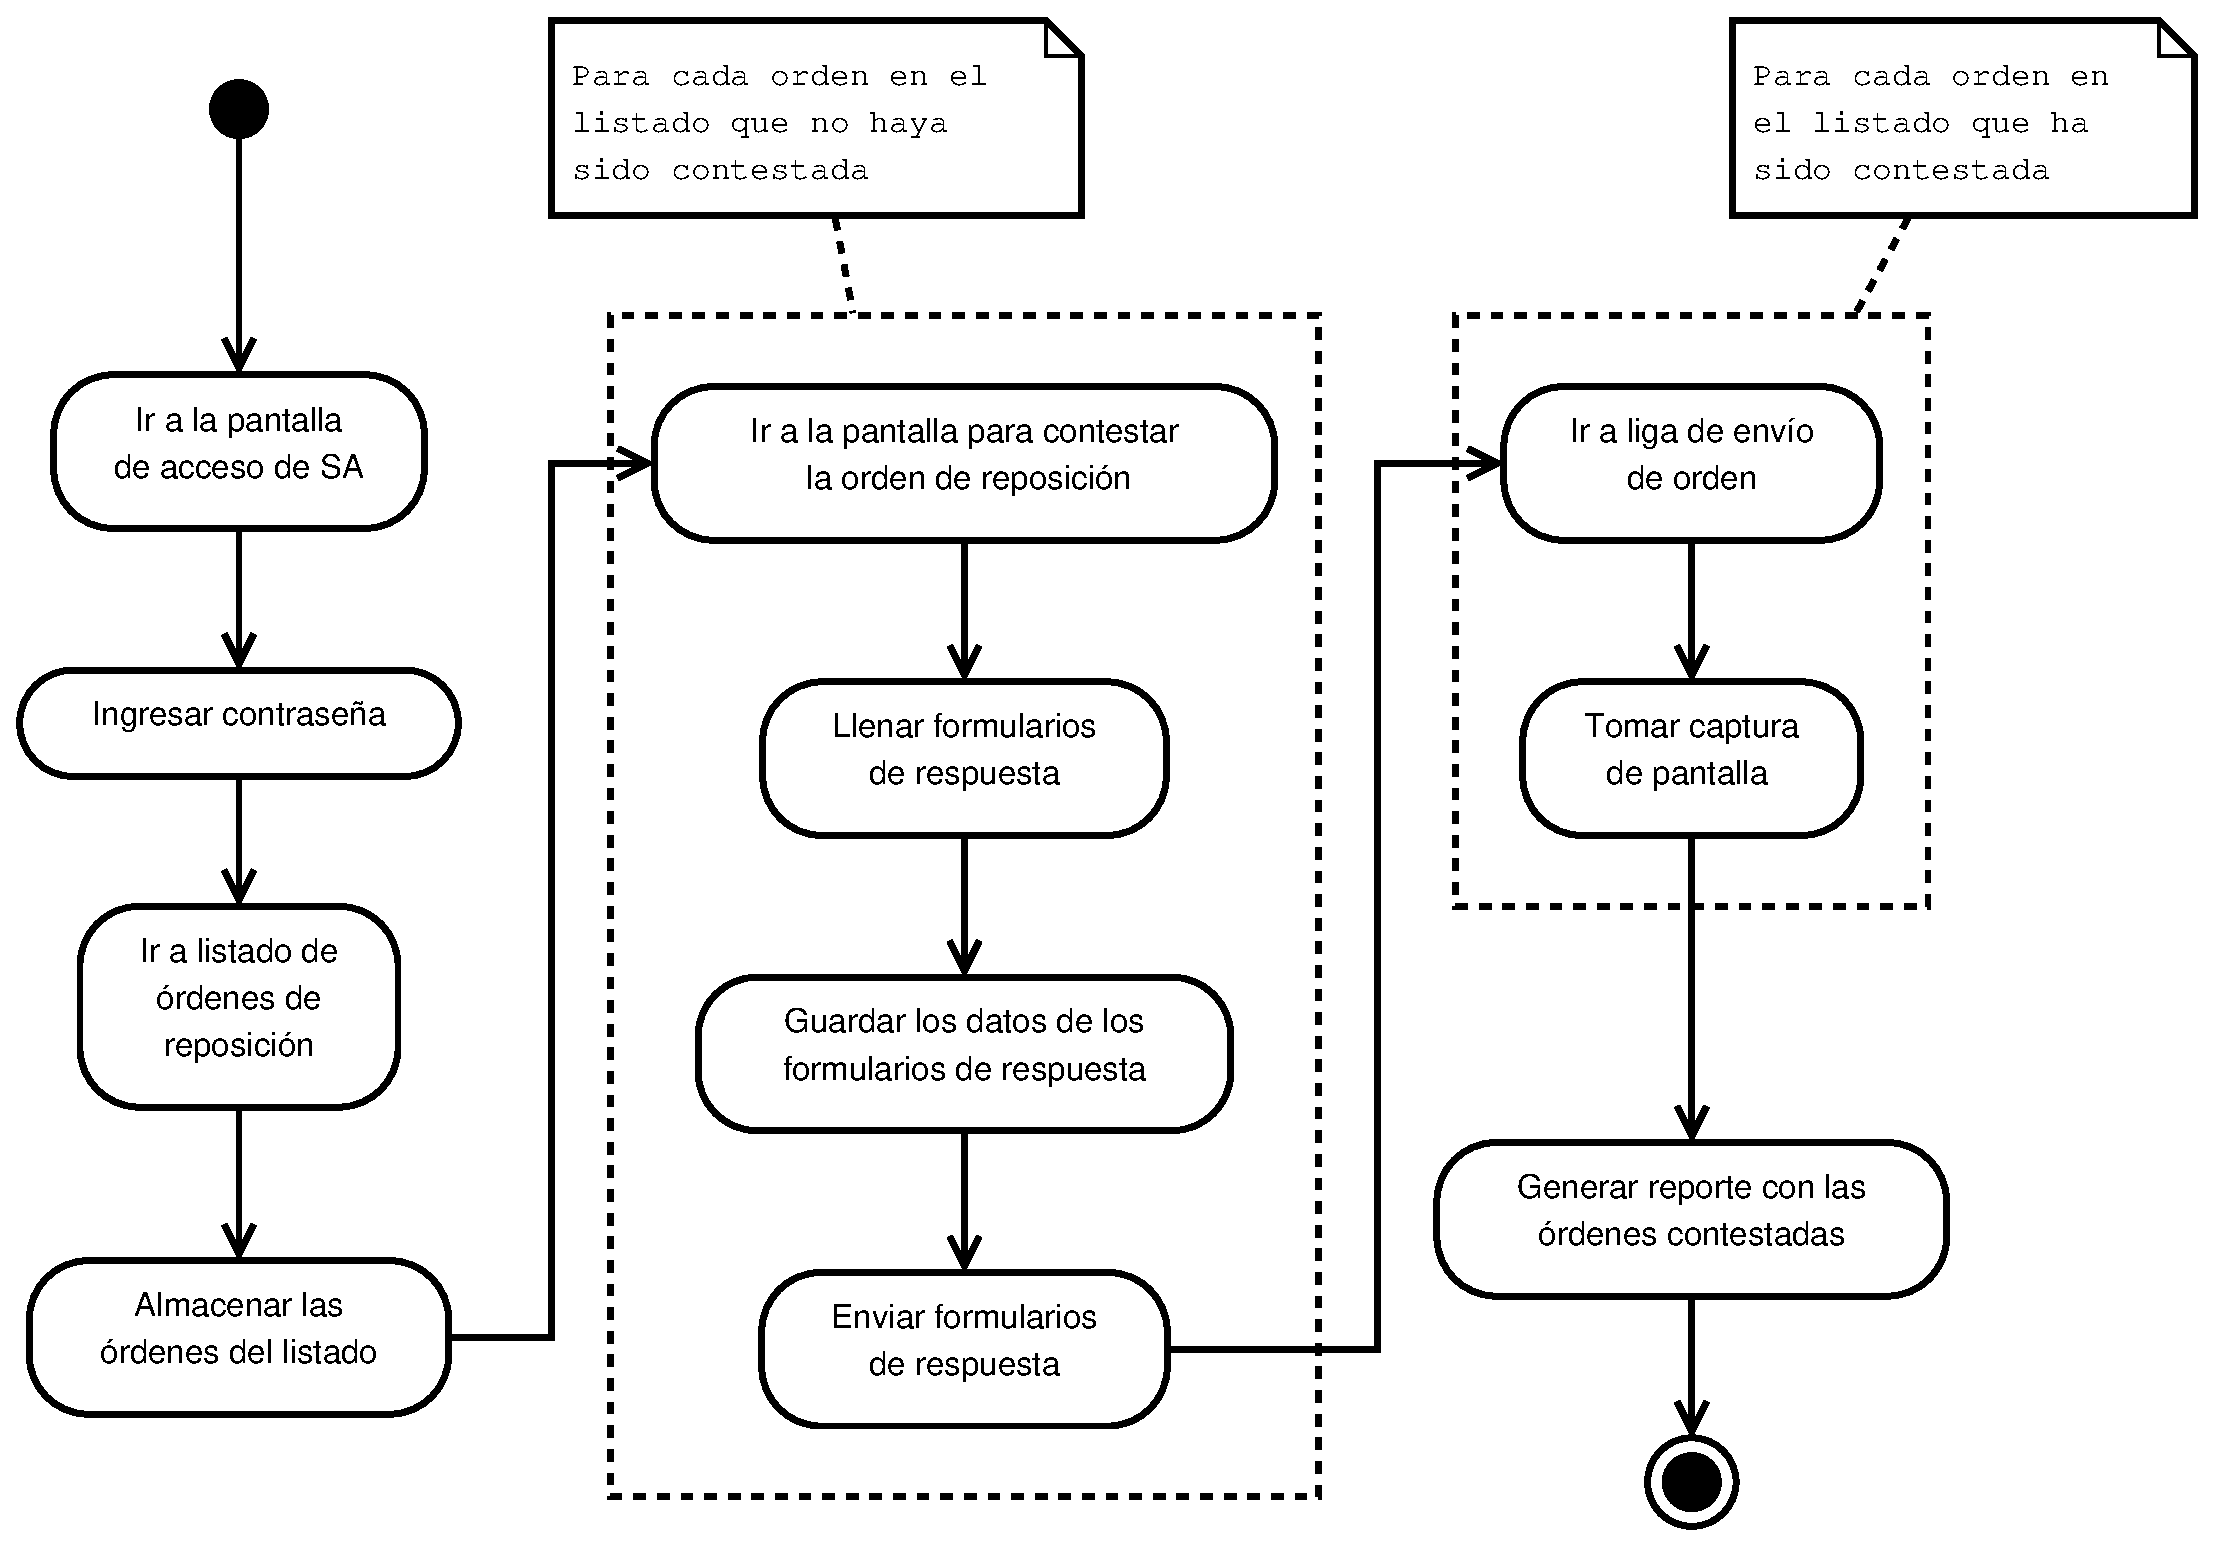
\includegraphics[scale=0.4]{dia-activity-contestar}
  \caption{Diagrama del proceso para contestar órdenes de reposición.}
  \label{fig:dia-activity-contestar}
\end{figure}

\subsubsection{Automatización del proceso para cotejar órdenes de reposición canceladas}\label{sec:req-verificar}
Automatizar la interacción del operador de la farmacéutica para conocer las órdenes de reposición que han sido canceladas recientemente por el \textit{Instituto}, como se muestra en el diagrama de proceso de negocio en la Figura \ref{fig:dia-activity-verificar} \footnote{
Ver también la Figura \ref{fig:flow-proc-verificar}.}.
\begin{figure}[h]
  \centering
  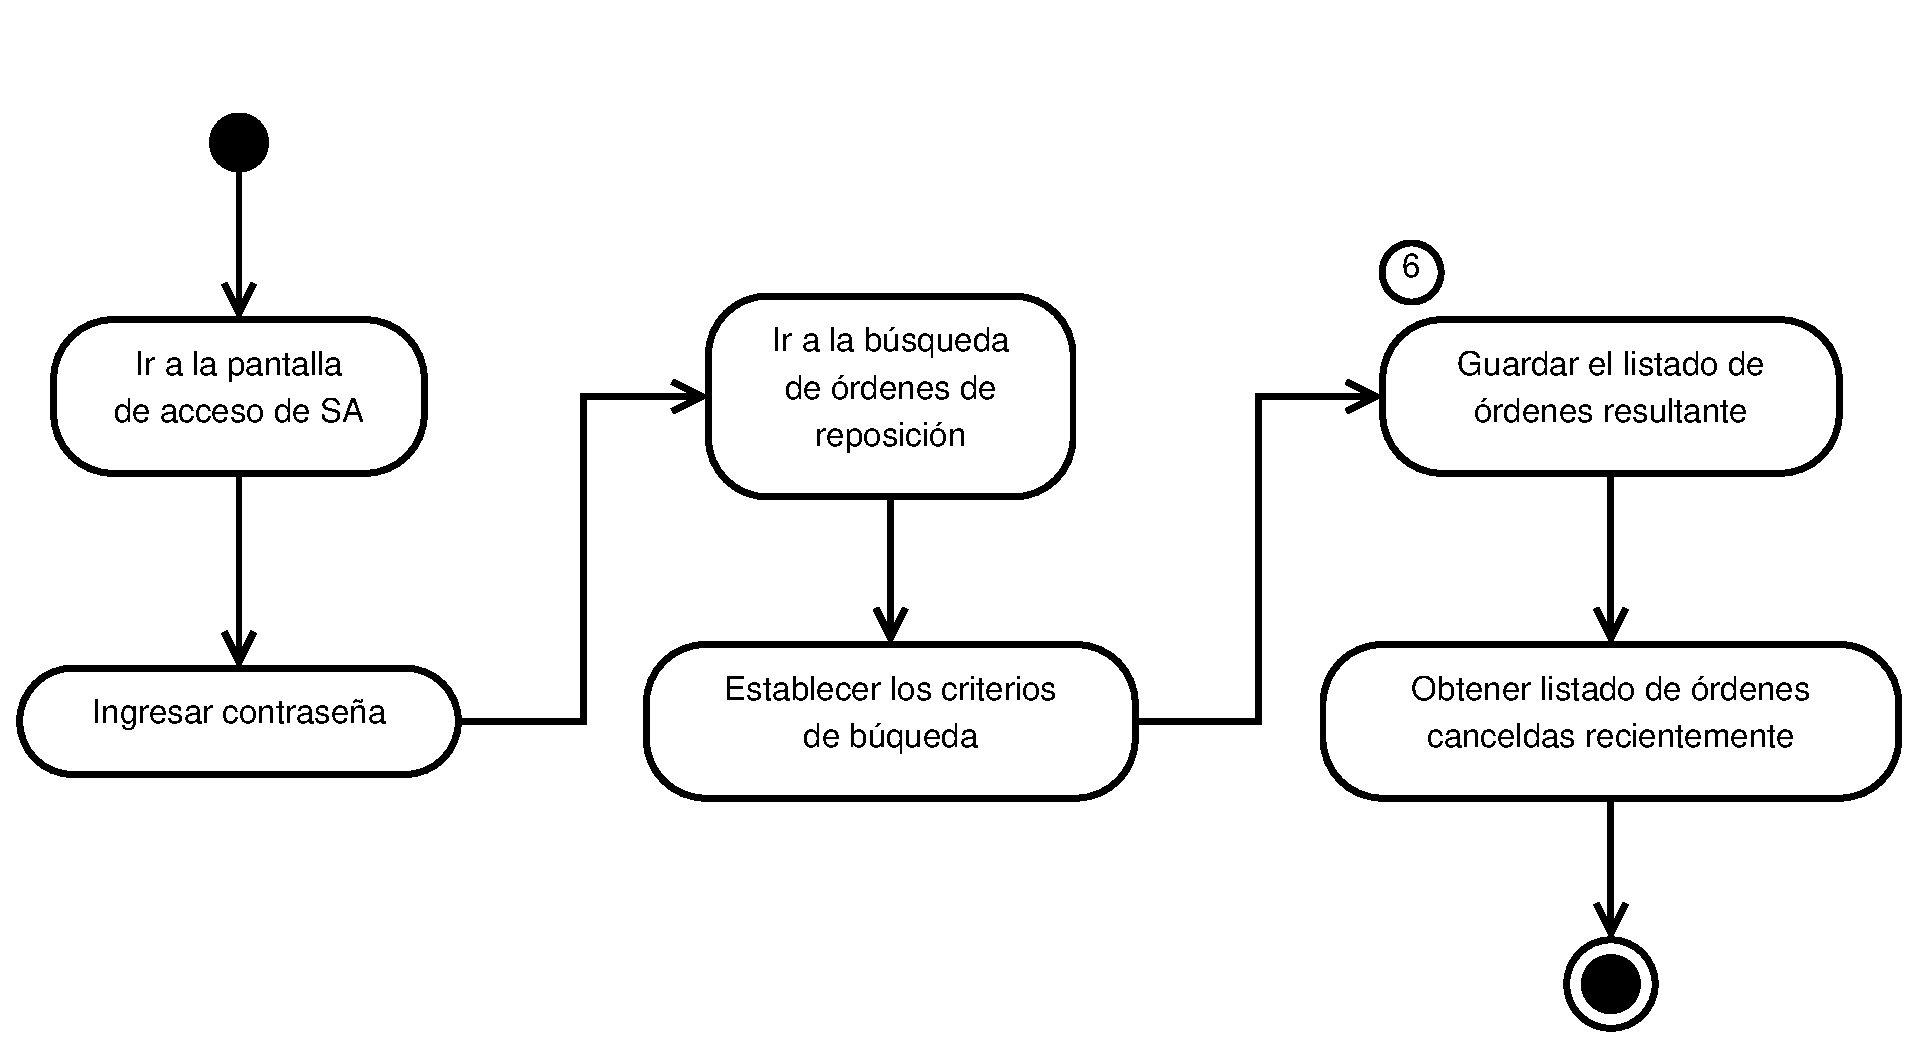
\includegraphics[scale=0.4]{dia-activity-verificar}
  \caption{Diagrama del proceso para verificar órdenes de reposición canceladas.}
  \label{fig:dia-activity-verificar}
\end{figure}
% espaciado
\pagebreak
% espaciado
\subsubsection{Interfaz web para la administración de órdenes de reposición contestadas}\label{sec:req-web-ui}
Todos los requerimientos de administración de órdenes de reposición y generación de reportes deben ser accedidos mediante una interfaz web protegida por nombre de usuario y contraseña\footnote{Excepto lo referente a los procesos automatizados de los operadores de la farmacéutica.}, como se muestra en la Figura \ref{fig:maq-login}.
\begin{figure}[h]
  \centering
  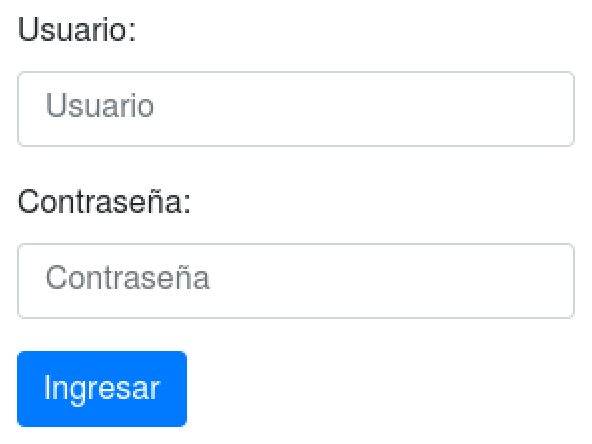
\includegraphics[scale=0.5]{maq-login} 
  \caption{Maqueta del acceso a la interfaz web.}
  \label{fig:maq-login}
\end{figure} 

\subsubsection{Búsqueda de órdenes de reposición}\label{sec:req-search}
En la interfaz web existe la posibilidad de buscar entre las órdenes de reposición contestadas mediante el número de orden de reposición. Esta opción entrega solo una orden de reposición. O bien, se puede utilizar un intervalo de fechas entre las cuales fueron atendidas tales órdenes, lo que entrega un listado de todas las órdenes de reposición que fueron respondidas en dicho intervalo. Las órdenes resultantes de la búsqueda deben ofrecer la opción para visualizar la información almacenada durante el proceso de respuesta, como se muestra en la Figura \ref{fig:maq-search}
\begin{figure}[h]
  \centering
  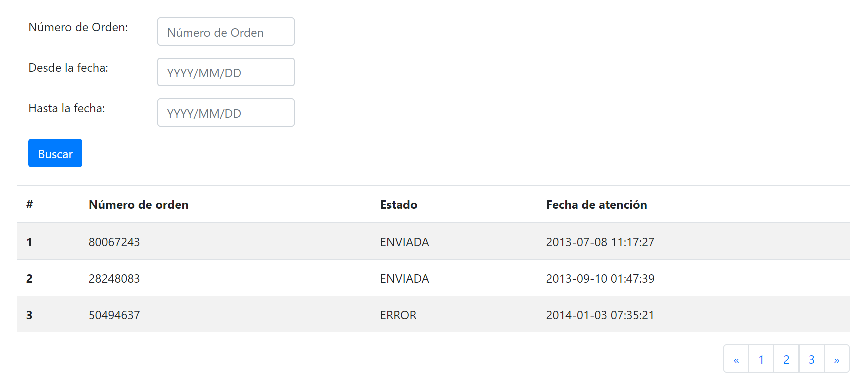
\includegraphics[width=\textwidth]{maq-search} 
  \caption{Maqueta de la búsqueda de órdenes.}
  \label{fig:maq-search}
\end{figure} 

\subsubsection{Visualización de orden de reposición}\label{sec:req-show}
La interfaz web tiene una sección donde se muestra el contenido de una orden de reposición almacenada en la base de datos (Figura \ref{fig:maq-crud}). Esta vista es individual, (no es posible mostrar el contenido de más de una orden de reposición), además, ofrece las opciones para modificar los datos de la orden (requerimiento \ref{sec:req-update}) y para generar el acuse de envío.
% espaciado
%\pagebreak
% espaciado
\begin{figure}[h]
  \centering
  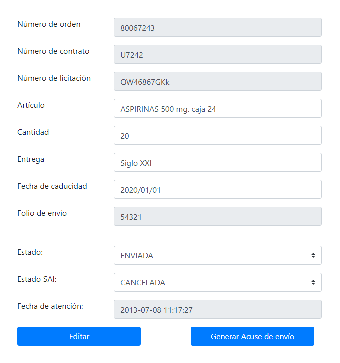
\includegraphics[scale=1]{maq-crud} 
  \caption{Maqueta del formulario para ver la información de una orden de reposición.}
  \label{fig:maq-crud}
\end{figure} 

\subsubsection{Edición de órdenes de reposición}\label{sec:req-update}
La interfaz web cuenta con una vista (similar a la forma de mostrar la información de una orden de reposición) que permite la modificación de una orden de reposición (Figura \ref{fig:maq-crud}). Esta vista es única (no es posible modificar más de una orden de reposición), por lo que no es posible modificar datos el número de orden y fecha de atención.

\subsubsection{Generación de reporte de órdenes de reposición contestadas}\label{sec:req-rep-contestadas}
El reporte con órdenes de reposición contestadas es acotado entre un par de fechas (con precisión de horas). Tal reporte (Figura \ref{fig:maq-report}), como su nombre lo indica, contiene los números de orden de reposición y datos definidos por la farmacéutica\footnote{Por acuerdo de confidencialidad, no se enunciarán los datos contenidos en los reportes.}
\begin{figure}[h]
  \centering
  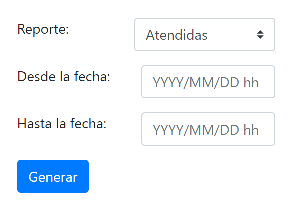
\includegraphics[scale=1.2]{maq-report} 
  \caption{Maqueta de la generación de reportes.}
  \label{fig:maq-report}
\end{figure} 

\subsubsection{Generación de formato de salida}\label{sec:req-rep-layout}
Este formato contiene los datos de las órdenes de reposición, las claves de los productos, así como los nombres de los centros de salud. El reporte (Figura \ref{fig:maq-report})\footnote{Por acuerdo de confidencialidad, no se enunciarán los datos contenidos en el formato de salida, tampoco el contenido de los catálogos de claves de producto y centros de salud.} está acotado entre un par de fechas (con precisión de horas).

\subsubsection{Generación de reporte con las órdenes de reposición canceladas \mbox{recientemente}}\label{sec:req-rep-canceladas}
Genera un reporte con las órdenes de reposición canceladas recientemente (Figura \ref{fig:maq-report}), es decir, las órdenes de reposición que tienen el estado de “cancelada” y no se han marcado como canceladas en el proceso de respuesta.

\subsubsection{Actualización de catálogos}\label{sec:req-catalogos}
Carga de forma masiva, mediante un archivo separado por comas (Figura \ref{fig:maq-upload}), los catálogos con claves de medicamentos, centros de salud y claves propias del manejo de la farmacéutica. Los catálogos definidos para la operación del sistema AutoSA no podrán ser actualizados; por ejemplo, los catálogos que contienen los estados posibles de una orden de reposición dentro del flujo de atención (Figura \ref{fig:dia-estados-orden}).
\begin{figure}[h]
  \centering
  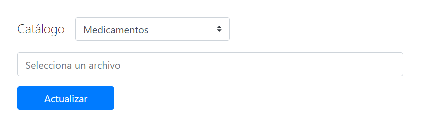
\includegraphics[scale=1.3]{maq-upload}
  \caption{Maqueta para la actualización de catálogos.}
  \label{fig:maq-upload}
\end{figure}

\subsubsection{Actualización de estatus de órdenes de reposición canceladas}\label{sec:req-canceladas}
Para realizar la actualización del estatus de las órdenes de reposición canceladas, el usuario carga al sistema un archivo de texto separado por comas, similar a la actualización de catálogos (Figura \ref{fig:dia-estados-orden}), con los números de las órdenes de reposición que han sido canceladas y se ha notificado al área correspondiente de la farmacéutica para cancelar la atención de dichas órdenes.

\subsubsection{Navegación dentro de la interfaz web}\label{sec:req-nav-bar}
La interfaz web muestra en todo momento un menú que permite la navegación entre las siguientes secciones (Figura \ref{fig:dia-nav-flow}):
\begin{enumerate}
  \item Generación de reportes.
  \item Actualización de catálogos (incluye la actualización de órdenes canceladas).
  \item Búsqueda de órdenes de reposición.
\end{enumerate}
\begin{figure}[h]
  \centering
  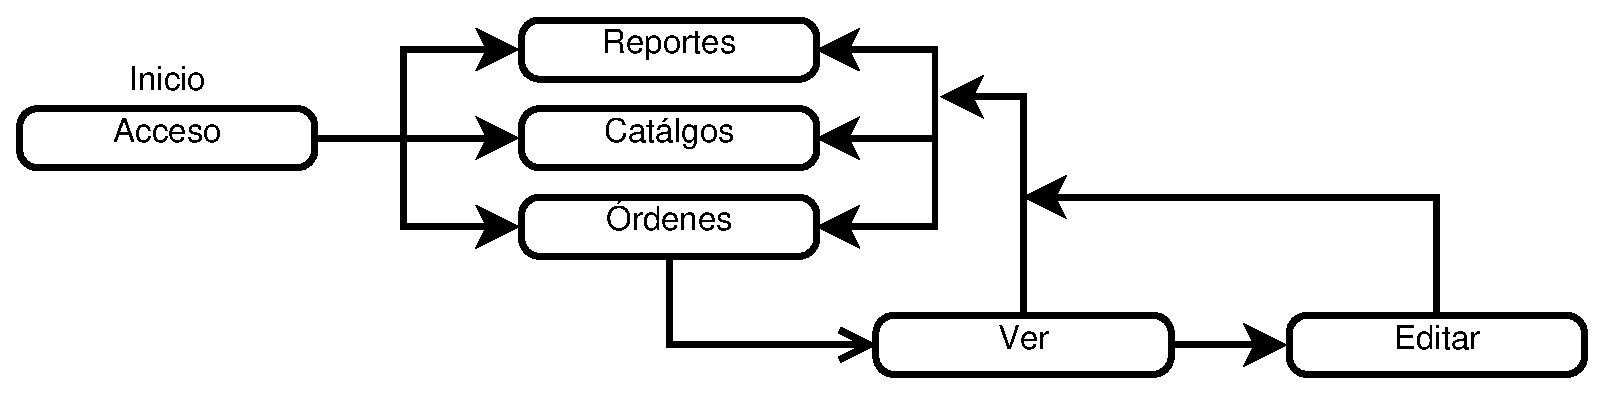
\includegraphics[scale=0.5]{dia-nav-flow}
  \caption{Mapa de navegación en la interfaz web.}
  \label{fig:dia-nav-flow}
\end{figure}


\subsection{Requerimientos no funcionales}\label{sec:nonfunctional-req}
Con el fin de evitar riesgos de seguridad informática, el cliente ha solicitado que el proyecto se apegue a su infraestructura\footnote{Por políticas de seguridad de la farmacéutica, no se enunciarán las herramientas e infraestructura utilizada, tampoco las versiones de las mismas.} además de cumplir con la siguientes especificaciones:
\begin{enumerate}
\item Capacidad del Sistema AutoSA para ser ejecutado en los sistemas operativos más comunes en la industria.
\item Base de datos relacional SQL.
\item Uso de la herramienta \textit{Sahi} para automatizar la interacción con el \textit{Sistema de Abastecimiento}.
\item Las contraseñas de los usuarios para el acceso a la interfaz web deben ser almacenadas utilizando un algoritmo de cifrado.
\end{enumerate}


%===============================================================================
%===============================================================================


\section{Casos de uso}\label{sec:casos-uso}
Un caso de uso es la representación de las posibles interacciones entre el sistema y sus actores, entendiendo un actor como una instancia (usuario u otro sistema). Asimismo, un caso de uso describe la funcionalidad del sistema por medio de mensajes y respuestas entre el actor y el sistema\cite{ApressSE}. En la Figura \ref{fig:dia-casos-uso} se muestra el diagrama de casos de uso del sistema AutoSA.

\begin{figure}[h]
  \centering
  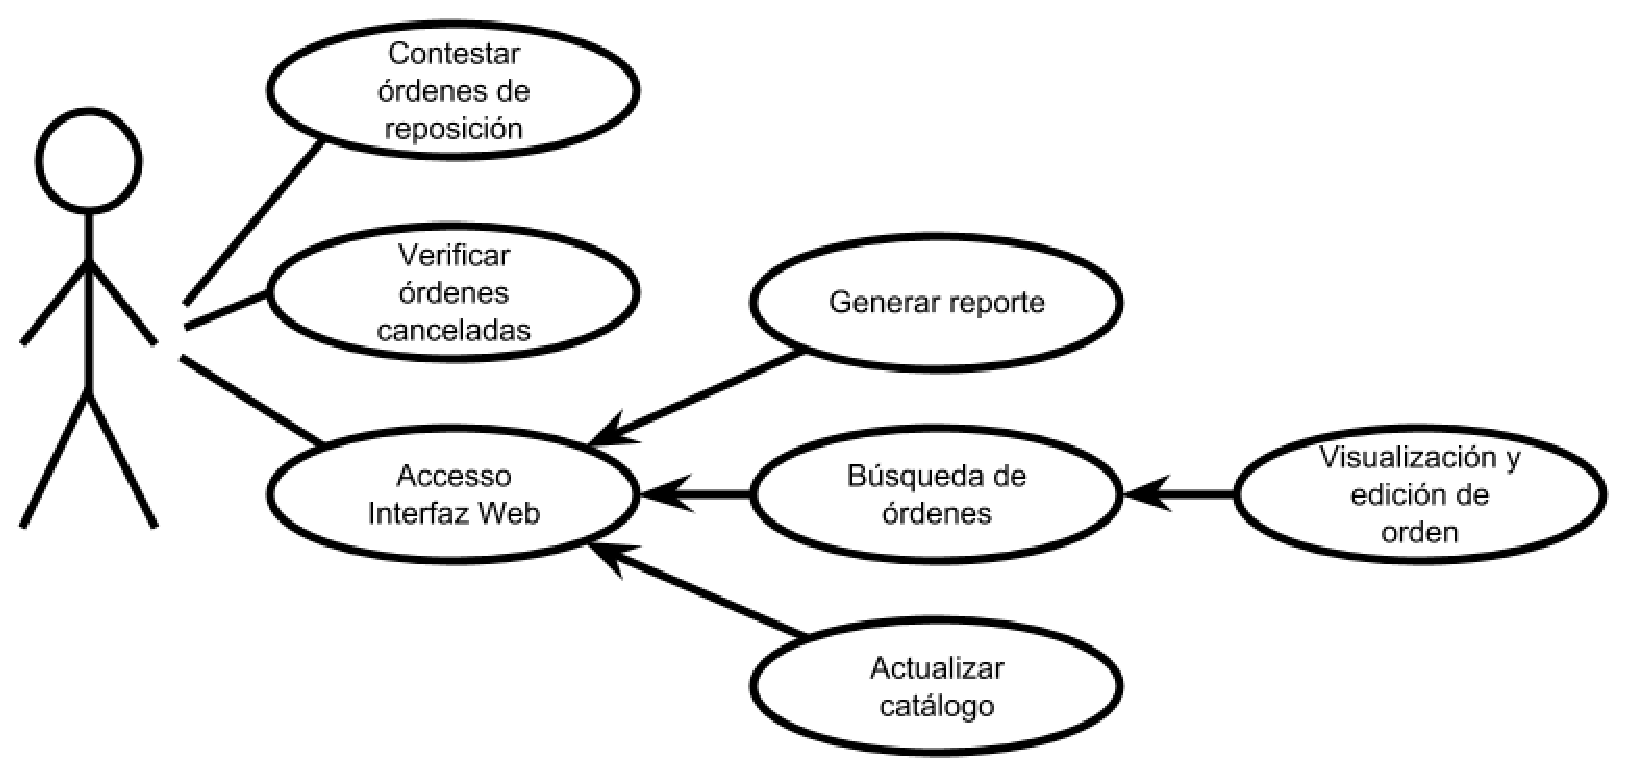
\includegraphics[width=\textwidth]{dia-casos-uso} 
  \caption{Diagrama de casos de uso.}
  \label{fig:dia-casos-uso}
\end{figure}

Con el fin de explicar mejor el flujo de atención de una orden de reposición, es necesario mostrar el diagrama de estados de una orden de reposición durante el flujo de \textbf{envío de órdenes de reposición} (sección \ref{sec:intro-contexto}).\\
Los estados que puede tomar una orden (Figura \ref{fig:dia-estados-orden}) indican:
\begin{itemize}
  \item Si la solicitud está lista para ser procesada: \texttt{Nueva} o \texttt{Contestada}.
  \item Si está siendo procesada: \texttt{Siendo Contestada} o \texttt{Siendo Enviada}.
  \item Si ha terminado el ciclo correctamente: \texttt{Enviada}.
  \item Si ha terminado el ciclo con errores: \texttt{Error}.
\end{itemize} 

\begin{figure}[h]
  \centering
  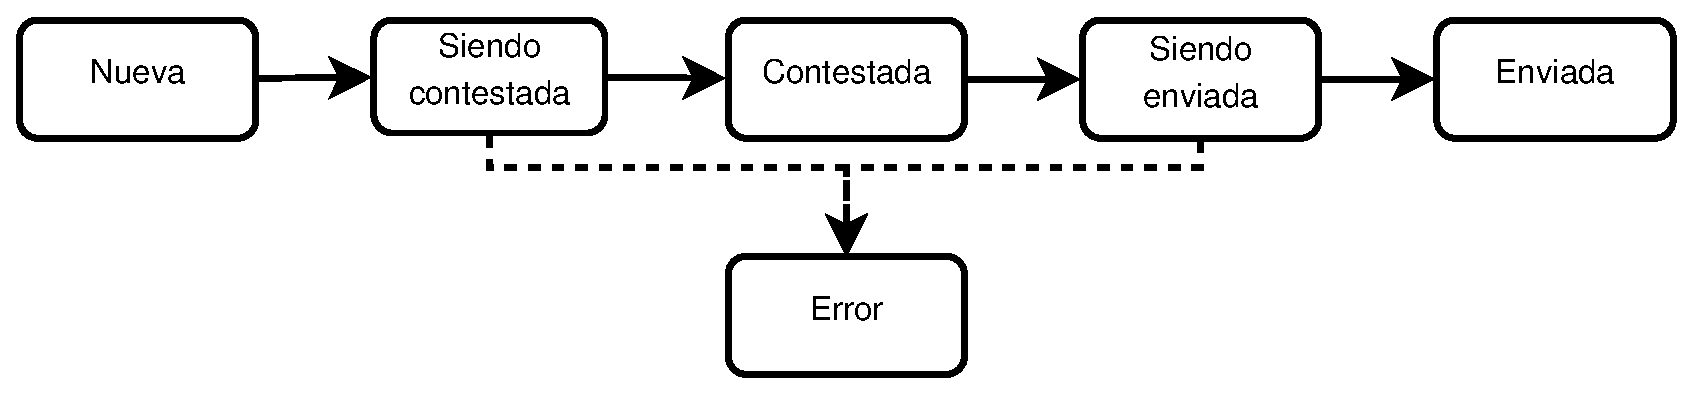
\includegraphics[width=\textwidth]{dia-estados-orden} 
  \caption{Diagrama de estados de una orden de reposición durante la rutina de respuesta de órdenes de reposición.}
  \label{fig:dia-estados-orden}
\end{figure}

Es importante mencionar que en las siguientes descripciones de caso de uso no se hará referencia al contenido exacto de las páginas, ni el nombre de los campos, únicamente se hará mención de los campos necesarios para dar una explicación clara del caso.

\subsection{Contestar órdenes}\label{cu-contestar}
\paragraph{Identificador:}
CU-CONTESTAR
\paragraph{Actores:}
Usuario
\paragraph{Descripción:}
El procedimiento principal para contestar las órdenes de reposición listadas en el \textit{Sistema de Abastecimiento} del \textit{Instituto Salud}, como se muestra en la Figura \ref{fig:dia-activity-contestar}, inicia con la consulta de la pantalla de acceso al \textit{Sistema de Abastecimiento}.\\
El alcance de este caso comprende el acceso al \textit{Sistema de Abastecimiento}: contestar y enviar las órdenes de reproducción almacenando los datos y generando la captura de pantalla de dichas órdenes.\\
Queda fuera de alcance la obtención del reporte con las órdenes de reposición que han sido canceladas recientemente. Es cubierto por el caso de uso Generación de Reportes.
\paragraph{Precondiciones:}
\begin{enumerate}
  \item El \textit{Sistema de Abastecimiento} se encuentra funcionando correctamente.
  \item El usuario cuenta con las credenciales para ingresar al \textit{Sistema de Abastecimiento}.
\end{enumerate}
\paragraph{Secuencia normal:}
\begin{enumerate}
  \item Inicia sesión en el \textit{Sistema de Abastecimiento}: provee nombre de usuario y solicita al usuario ingresar la contraseña.
  \item Dirige el explorador a la pantalla donde se encuentra el listado con las órdenes de reposición que no han sido contestadas.
  \item Para cada orden de reposición del listado que se muestra se aplica el caso de uso \textbf{CU-GUARDAR-NUEVA}.
  \item Para cada solicitud en la base de datos con estado \textbf{Nueva} se aplican los casos de uso:
  \begin{enumerate}
    \item \textbf{CU-RESPONDER-ORDEN}.
  \end{enumerate}
  \item Para cada solicitud con estatus \textbf{Contestada}:
  \begin{enumerate}
    \item \textbf{CU-ENVIAR-ORDEN}.
    \item \textbf{CU-GENERAR-ACUSE}.
  \end{enumerate}
  \item El programa se repite desde el paso 2 hasta terminar las solicitudes sin contar las marcadas con estatus \textbf{Error}.
  \item Registra el fin del procedimiento en la base de datos.
\end{enumerate}
\paragraph{Postcondiciones:}
\begin{enumerate}
  \item Todas las órdenes de reposición listadas han sido contestadas y enviadas.
  \item Se han registrado todas las órdenes de reposición atendidas en la base de datos.
  \item Los acuses de envió de las órdenes de reposición se encuentran en el sistema de archivos.
\end{enumerate}
\paragraph{Excepciones:}
\begin{enumerate}
  \item Si en algún momento se detecta la pérdida de sesión en la página del \textit{Sistema de Abastecimiento}, se reinicia el procedimiento desde el paso 1 de este caso de uso.
  \item Cualquier error durante la ejecución de este caso de uso será registrado en la bitácora el sistema.
\end{enumerate}


\subsection{Guardar nueva orden}\label{cu-guardar-nueva}
\paragraph{Identificador:}
CU-GUARDAR-NUEVA
\paragraph{Actores:}
Robot
\paragraph{Descripción:}
Una orden de reposición es almacenada por primera vez con la información que se muestra en el listado de órdenes de reposición. Este caso de uso corresponde a la actividad 4 del diagrama de actividad de la Figura \ref{fig:dia-activity-contestar}.
\paragraph{Precondiciones:}
\begin{enumerate}
  \item Se tiene indicado un renglón del listado de órdenes de reposición sobre el cual se realizará este caso de uso.
\end{enumerate}
\paragraph{Secuencia normal:}
\begin{enumerate}
  \item Del listado de órdenes de reposición, cada solicitud es ingresada a la base de datos con estatus \textbf{Nueva} y datos provenientes del listado:
  \begin{enumerate}
    \item Contrato.
    \item Solicitud.
    \item Número de orden.
    \item Fecha de expedición.
    \item Almacén destino.
    \item URL de respuesta.
    \item URL de envío: generada reemplazando el parámetro en la URL de respuesta ``responde'' por ``envia''\footnote{Dado que es una palabra en una URL no es recomendable el uso de acentos, por lo tanto se escribe ``envia'' y no ``envía''.}.
  \end{enumerate}
\end{enumerate}
\paragraph{Postcondiciones:}
\begin{enumerate}
  \item La orden de reposición se encuentra almacenada en la base de datos.
\end{enumerate}
\paragraph{Excepciones:}
\begin{enumerate}
  \item Si el listado muestra la URL de envío y la orden no ha sido almacenada, la orden es almacenada con estado \textbf{Contestada} y se registra \textbf{cantidad solicitada} igual a 0.
  \item Si ocurre algún error la orden es almacenada con estado \textbf{Error}.
\end{enumerate}


\subsection{Responder orden}\label{cu-responder-orden}
\paragraph{Identificador:}
CU-RESPONDER-ORDEN
\paragraph{Actores:}
Robot
\paragraph{Descripción:}
En la pantalla para contestar una orden de reposición se llenan los formularios y se almacena la información de la pantalla en el registro de la base de datos que corresponde a la orden de reposición. Este caso de uso corresponde a las actividades 6 y 7 del diagrama de actividad de la Figura \ref{fig:dia-activity-contestar}.
\paragraph{Precondiciones:}
\begin{enumerate}
  \item Se indica una orden de reposición almacenada en la base de datos sobre la cual se aplica este caso de uso.
  \item La orden de reposición se encuentra almacenada en la base de datos.
  \item La orden de reposición tiene estado \textbf{Nueva}.
\end{enumerate}
\paragraph{Secuencia normal:}
\begin{enumerate}
  \item Obtiene la orden de reposición y cambia el estado a \textbf{Siendo Contestada}, todo en una misma transacción.
  \item Dirige el explorador a la URL de respuesta (caso de uso \textbf{CU-GUARDAR-NUEVA}).
  \item Llena el formulario que se presenta en esta pantalla con las siguientes consideraciones:
  \begin{enumerate}
    \item Fecha de fabricación:
    \begin{itemize}
      \item Si el mes de la fecha actual es diciembre, entonces la fecha de fabricación es el 1 de enero del año siguiente.
      \item En caso contrario (el mes de la fecha actual no es diciembre), entonces la fecha de fabricación es el 1 de enero del año actual.
    \end{itemize}
    \item Fecha de caducidad: último día del año en curso, si la fecha actual no es del mes de diciembre; en caso contrario se toma el año siguiente.
    \begin{itemize}
      \item Si el mes de la fecha actual es diciembre, entonces la fecha de caducidad es el 31 de diciembre del año siguiente.
      \item En caso contrario (el mes de la fecha actual no es diciembre), entonces la fecha de caducidad es el 31 de diciembre del año actual.
    \end{itemize}
  \end{enumerate}
  \item Almacena en la base de datos los campos de los formularios.
  \item Cambia el estado de la orden a \textbf{Contestada}.
  \item Activa el botón ``contestar'' del formulario de la orden de reposición.
\end{enumerate}
\paragraph{Postcondiciones:}
\begin{enumerate}
  \item Los formularios de la pantalla han sido completados correctamente.
  \item Los datos del formulario se encuentran almacenado en la base de datos.
  \item El estado de la orden en la base de datos es \textbf{Contestada}.
\end{enumerate}
\paragraph{Excepciones:}
\begin{enumerate}
  \item Si ocurre algún error la orden es almacenada con estado \textbf{Error}.
\end{enumerate}


\subsection{Enviar orden}\label{cu-enviar-orden}
\paragraph{Identificador:}
CU-ENVIAR-ORDEN
\paragraph{Actores:}
Robot
\paragraph{Descripción:}
Enviar la orden de reposición contestada de regreso al \textit{Sistema de Abastecimiento}. Este caso de uso corresponde a las actividades 8 y 9 del diagrama de actividad de la Figura \ref{fig:dia-activity-contestar}.
\paragraph{Precondiciones:}
\begin{enumerate}
  \item Una orden de reposición registrada en la base de datos.
  \item La orden de reposición tiene estado \textbf{Contestada}.
\end{enumerate}
\paragraph{Secuencia normal:}
\begin{enumerate}
  \item Cambia estado de la orden a \textbf{Siendo Enviada}.
  \item Dirige el explorador a la \textit{URL de envío}.
  \item Guardar el folio de envío en la base de datos.
  \item Cambia estado de la orden a \textbf{Enviada}.
\end{enumerate}
\paragraph{Postcondiciones:}
\begin{enumerate}
  \item El folio de envío de la orden de reposición se encuentra guardado en la base datos.
  \item El estado de la orden en la base de datos es \textbf{Enviada}.
\end{enumerate}
\paragraph{Excepciones:}
\begin{enumerate}
  \item Si ocurre algún error la orden es almacenada con estado \textbf{Error}.
\end{enumerate}


\subsection{Generar acuse de envío}\label{cu-generar-acuse}
\paragraph{Identificador:}
CU-GENERAR-ACUSE
\paragraph{Actores:}
Robot
\paragraph{Descripción:}
Generar el acuse de envío de la orden de reposición. Este caso de uso corresponde a la actividad 10 del diagrama de actividad de la Figura \ref{fig:dia-activity-contestar}.
\paragraph{Precondiciones:}
\begin{enumerate}
  \item Una orden de reposición registrada en la base de datos.
  \item La orden de reposición tiene estado \textbf{Enviada}.
\end{enumerate}
\paragraph{Secuencia normal:}
\begin{enumerate}
  \item Extraer la información de la orden de reposición de la base de datos.
  \item Mandar la generación del acuse de envío.
  \item Colocar el documento generado en el sistema de archivos.
\end{enumerate}
\paragraph{Postcondiciones:}
\begin{enumerate}
  \item Un documento en el sistema de archivos que contiene el acuse de envío.
\end{enumerate}
\paragraph{Excepciones:}
\begin{enumerate}
  \item En caso de algún error, se registra el error en la bitácora del sistema (el usuario posteriormente podrá volver a imprimir el acuse. Ver caso de uso \textbf{CU-VISUALIZAR}).
\end{enumerate}


\subsection{Verificar órdenes}\label{cu-verificar}
\paragraph{Identificador:}
CU-VERIFICAR
\paragraph{Actores:}
Usuario
\paragraph{Descripción:}
Modelar el procedimiento automatizado para verificar órdenes de reposición canceladas. En la Figura \ref{fig:dia-activity-verificar} se muestra que dicho procedimiento comienza con la actividad de mostrar la página de acceso al \textit{Sistema de Abastecimiento} para después dirigirse a la página donde se realiza la búsqueda de órdenes de reposición por estado (Contestada, Enviada, Cancelada).\\
El alcance de este caso de uso comprende el acceso al \textit{Sistema de Abastecimiento}, búsqueda de órdenes de reposición con estado \textbf{Cancelado} y comparación con la base de datos.\\
Quedan fuera de alcance: la actualización masiva del estado de órdenes de reposición (es cubierto en el caso de uso \textbf{CU-ACTUALIZAR-CATALOGO}) y la obtención del reporte con las órdenes de reposición que han sido canceladas recientemente (es cubierto por el caso de uso \textbf{CU-GENERAR-REPORTE}).
\paragraph{Precondiciones:}
\begin{enumerate}
  \item El \textit{Sistema de Abastecimiento} se encuentra funcionando correctamente.
  \item El usuario cuenta con las credenciales para ingresar al \textit{Sistema de Abastecimiento}.
\end{enumerate}
\paragraph{Secuencia normal:}
\begin{enumerate}
  \item Inicia sesión en el \textit{Sistema de Abastecimiento}: provee nombre de usuario y le solicita al usuario ingresar la contraseña.
  \item Dirige el explorador a la pantalla de búsqueda de órdenes de reposición.
  \item Llena el formulario para el filtro de búsqueda:
  \begin{enumerate}
    \item Rango de fechas que comprende los últimos siete días desde la fecha actual.
    \item Estado \textbf{Cancelada}.
  \end{enumerate}
  \item Del listado de órdenes de reposición resultantes se genera una lista con el número de orden de cada renglón.
  \item Con el listado del paso anterior se realiza el caso de uso \textbf{CU-ACTUALIZAR-ESTATUS-SA}.
\end{enumerate}
\paragraph{Postcondiciones:}
\begin{enumerate}
  \item Se cuenta con la relación de órdenes de reposición atendidas por el sistema que han sido canceladas en el \textit{Sistema de Abastecimiento} y no se tenía conocimiento previo.
  \item Las órdenes de reposición publicadas en el \textit{Sistema de Abastecimiento} dentro de los últimos siete días a la fecha actual reflejan en la base de datos dentro del campo \textbf{EstadoSA}\footnote{Este campo refleja el estado de atención registrado dentro del \textit{Sistema de Abastecimiento}.}.
\end{enumerate}
\paragraph{Excepciones:}
\begin{enumerate}
  \item Cualquier error durante la ejecución de este caso de uso será registrado en la bitácora el sistema.
\end{enumerate}


\subsection{Actualizar estatus de Sistema de Abastecimiento}\label{cu-actualizar-estatus-sa}
\paragraph{Identificador:}
CU-ACTUALIZAR-ESTATUS-SA
\paragraph{Actores:}
Robot
\paragraph{Descripción:}
Actualizar en forma masiva el estado de atención en el \textit{Sistema de Abastecimiento} dentro de la base de datos del sistema AutoSA. Este caso de uso corresponde a la actividad 6 del diagrama de actividad de la Figura \ref{fig:dia-activity-verificar}.
\paragraph{Precondiciones:}
\begin{enumerate}
  \item Se cuenta con una lista de órdenes de reposición.
  \item Las órdenes listadas tienen estado \textbf{Cancelada} en el \textit{Sistema de Abastecimiento}. 
\end{enumerate}
\paragraph{Secuencia normal:}
\begin{enumerate}
  \item Actualiza el estado \texttt{Sistema de Abastecimiento} de las órdenes de reposición en la base de datos.
\end{enumerate}
\paragraph{Postcondiciones:}
\begin{enumerate}
  \item Las órdenes de reposición recibidas tienen estado \textbf{Cancelada} en el campo \textbf{EstadoSA} dentro de la base de datos.
\end{enumerate}
\paragraph{Excepciones:}
\begin{enumerate}
  \item Las órdenes de reposición que no estén registradas en la base de datos se registrarán con campos nulos a excepción del número de orden.
  \item Cualquier error durante la ejecución de este caso de uso será registrado en la bitácora el sistema.
\end{enumerate}


\subsection{Entrar en interfaz web}\label{cu-entrar-web}
\paragraph{Identificador:}
CU-ENTRAR-WEB
\paragraph{Actores:}
Usuario
\paragraph{Descripción:}
Este caso de uso define el flujo para autorizar la entrada de un usuario a la interfaz web del sistema. En el diagrama de actividad de la Figura \ref{fig:dia-activity-login} se puede observar que el flujo inicia cuando el sistema muestra la pantalla de acceso (parte superior izquierda del apartado AutoSA). Este es el punto de acceso que tienen los usuarios para hacer acciones de administración de las órdenes de reposición atendidas por las rutinas de automatización, generación de reportes y actualización de catálogos.
\begin{figure}[h]
  \centering
  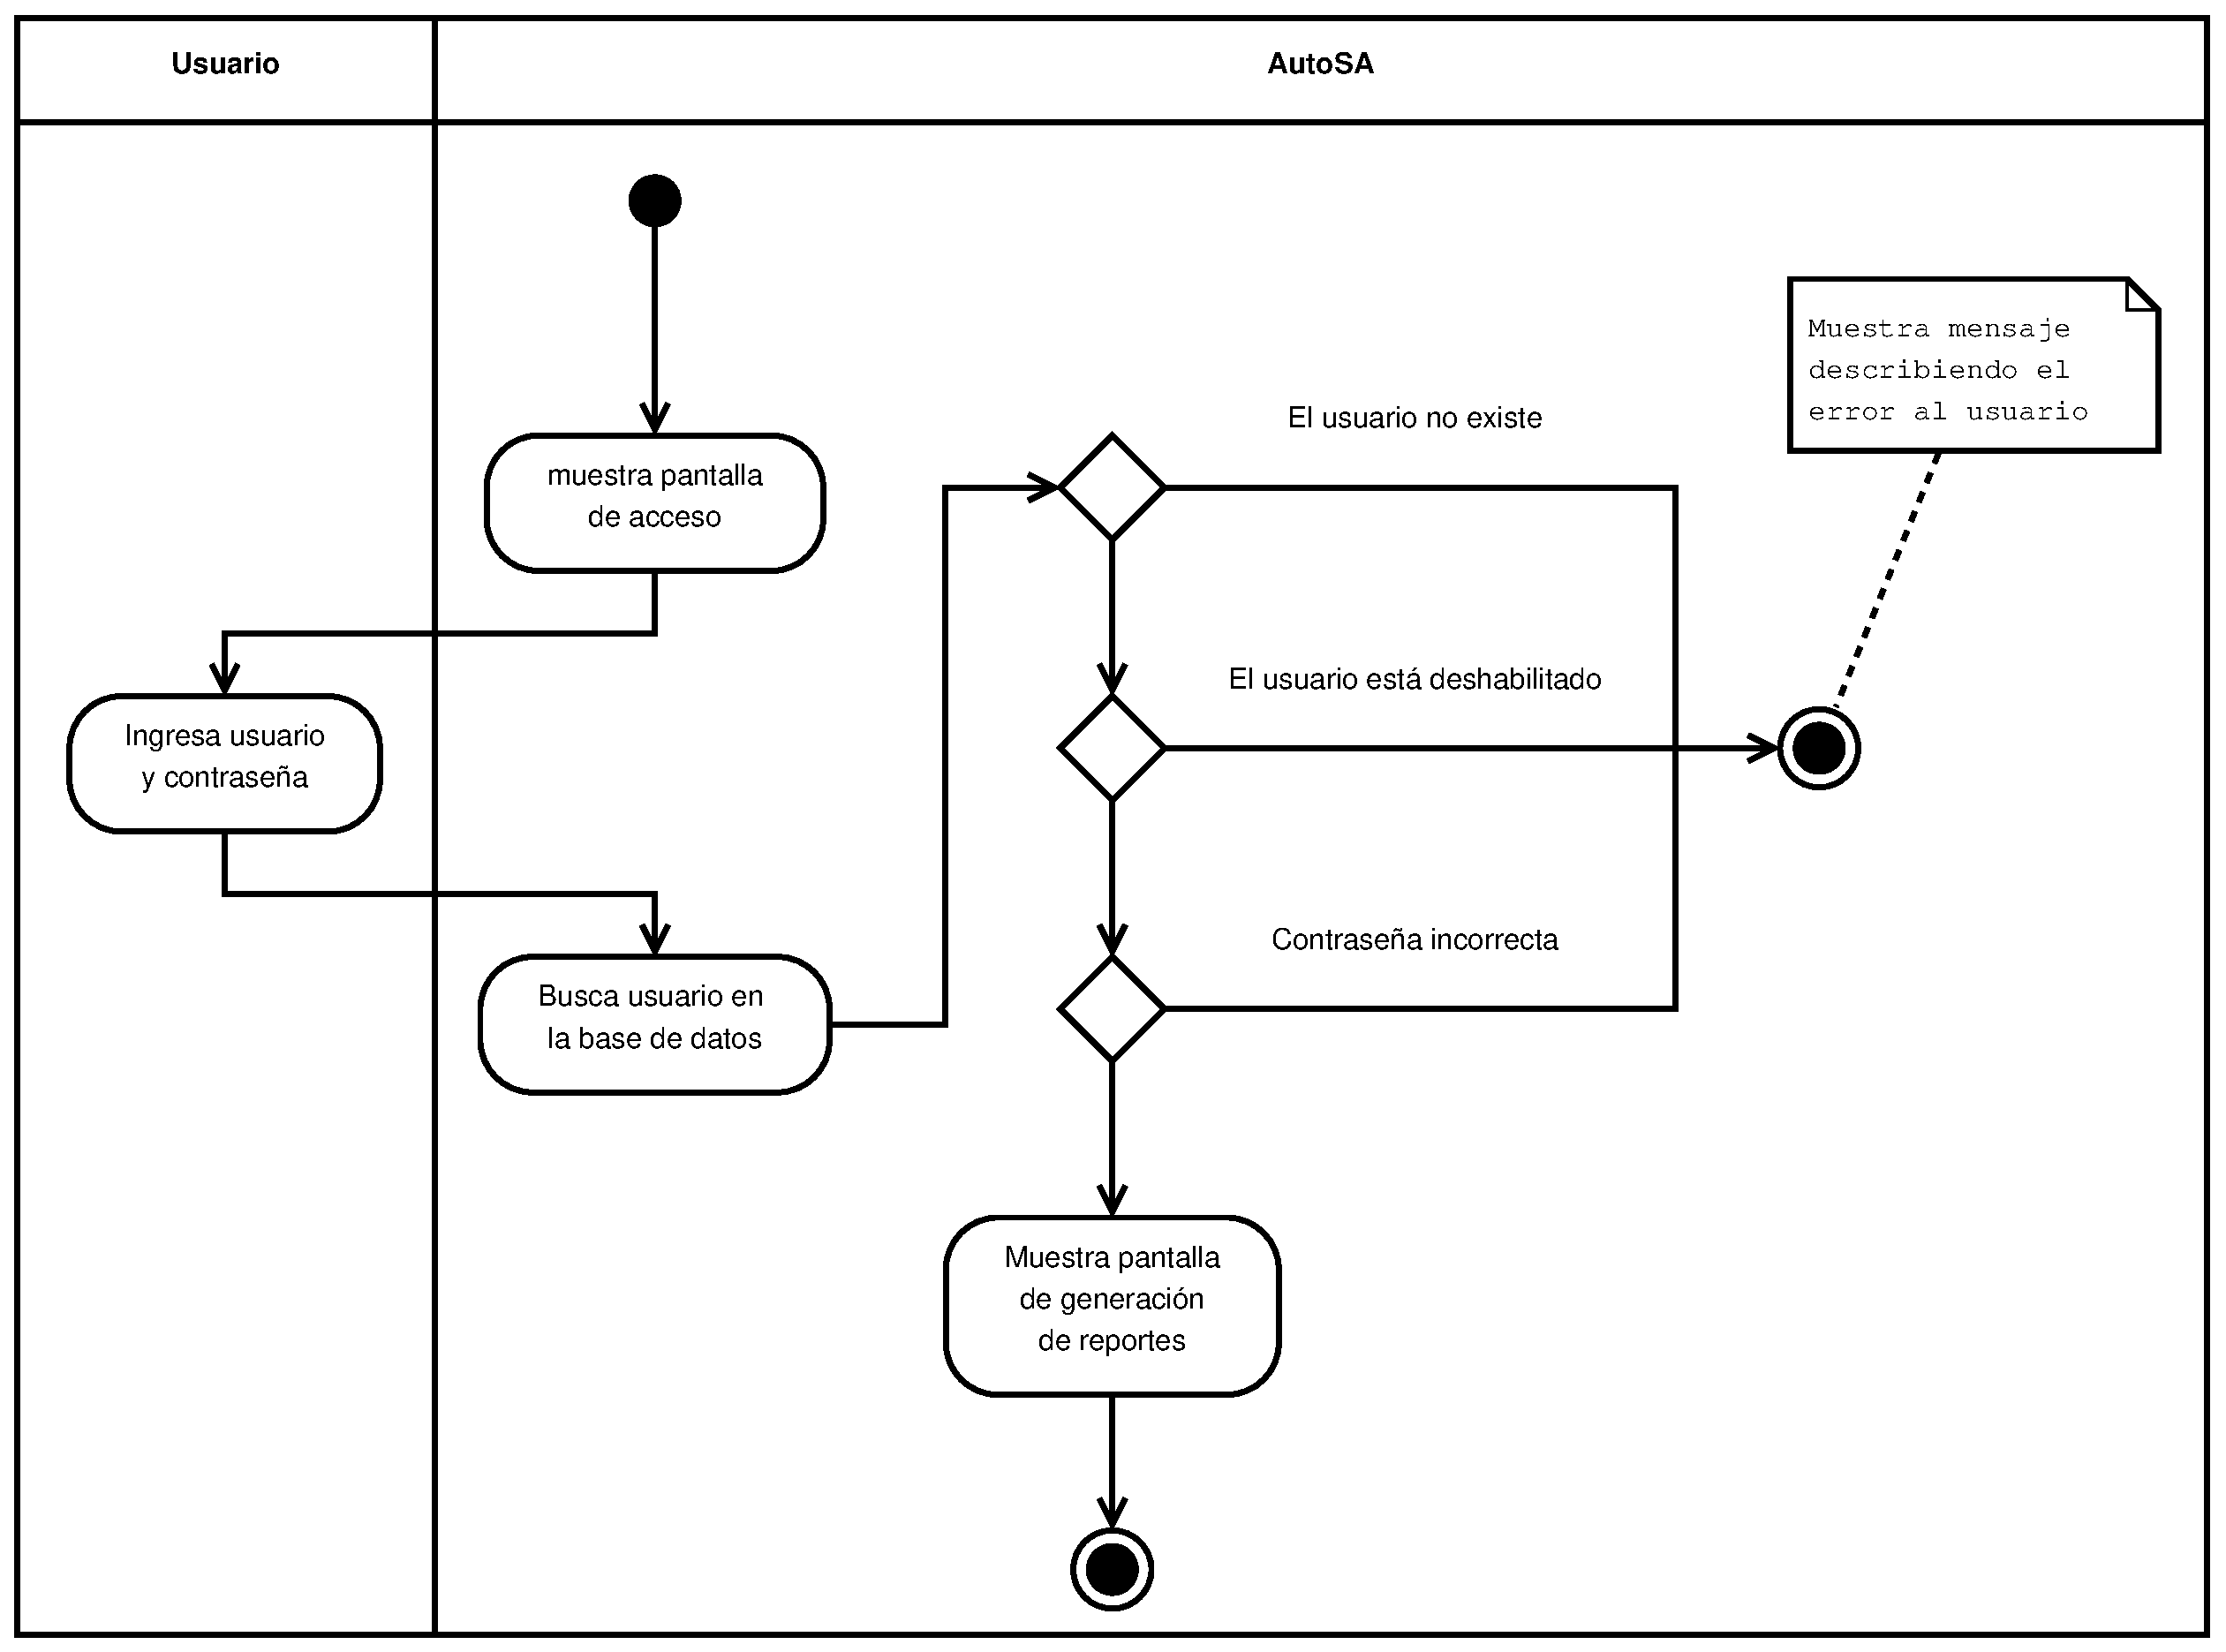
\includegraphics[width=\textwidth]{dia-activity-login}
  \caption{Diagrama de actividad del flujo de acceso al sistema.}
  \label{fig:dia-activity-login}
\end{figure}
\paragraph{Precondiciones:}
\begin{enumerate}
  \item El usuario solicita la página de acceso al sistema web.
\end{enumerate}
%espaciado
%\pagebreak
%espaciado
\paragraph{Secuencia normal:}
\begin{enumerate}
  \item El sistema muestra la pantalla de acceso.
  \item El usuario ingresa los campos:
  \begin{enumerate}
    \item Nombre de usuario.
    \item Contraseña.
  \end{enumerate}
  \item El sistema busca el nombre de usuario en la base de datos.
  \item El sistema compara la contraseña provista por el usuario con el valor almacenado en la base de datos.
  \item Muestra la pantalla de generación de reportes.
\end{enumerate}
\paragraph{Postcondiciones:}
\begin{enumerate}
  \item El usuario cuenta con un código temporal de acceso a la interfaz web.
  \item Se muestra la pantalla de generación de reportes.
\end{enumerate}
\paragraph{Excepciones:}
\begin{enumerate}
  \item Los siguientes escenarios se consideran un error de autenticación:
  \begin{itemize}
    \item El usuario no existe en la base de datos.
    \item El usuario tiene estado \textbf{deshabilitado}.
    \item La contraseña proporcionada no coincide con la almacenada. 
  \end{itemize}
\end{enumerate}

\subsection{Generar reporte}\label{cu-generar-reporte}
\paragraph{Identificador:}
CU-GENERAR-REPORTE
\paragraph{Actores:}
Usuario
\paragraph{Descripción:}
Este caso de uso ofrece al usuario la generación de reportes, entendiendo como reporte un documento de \textit{Excel}\textsuperscript{\textcopyright} que contiene el resultado de una consulta a la base de datos.\\
En el diagrama de actividad de la Figura \ref{fig:dia-activity-reporter} se muestra el flujo que sigue este caso de uso, el cual comienza con el usuario solicitando la pantalla para la generación de reportes (parte superior del apartado Usuario del diagrama de actividad).\\
Es posible que la consulta a la base de datos (primera actividad del apartado AutoSA del diagrama de actividad) haga referencia a catálogos con claves de productos y clientes que cambian constantemente, por lo que es necesario considerar la actualización de catálogos. Tal funcionalidad es cubierta por el caso de uso \textbf{CU-ACTUALIZAR-CATALOGO}.
\begin{figure}[h]
  \centering
  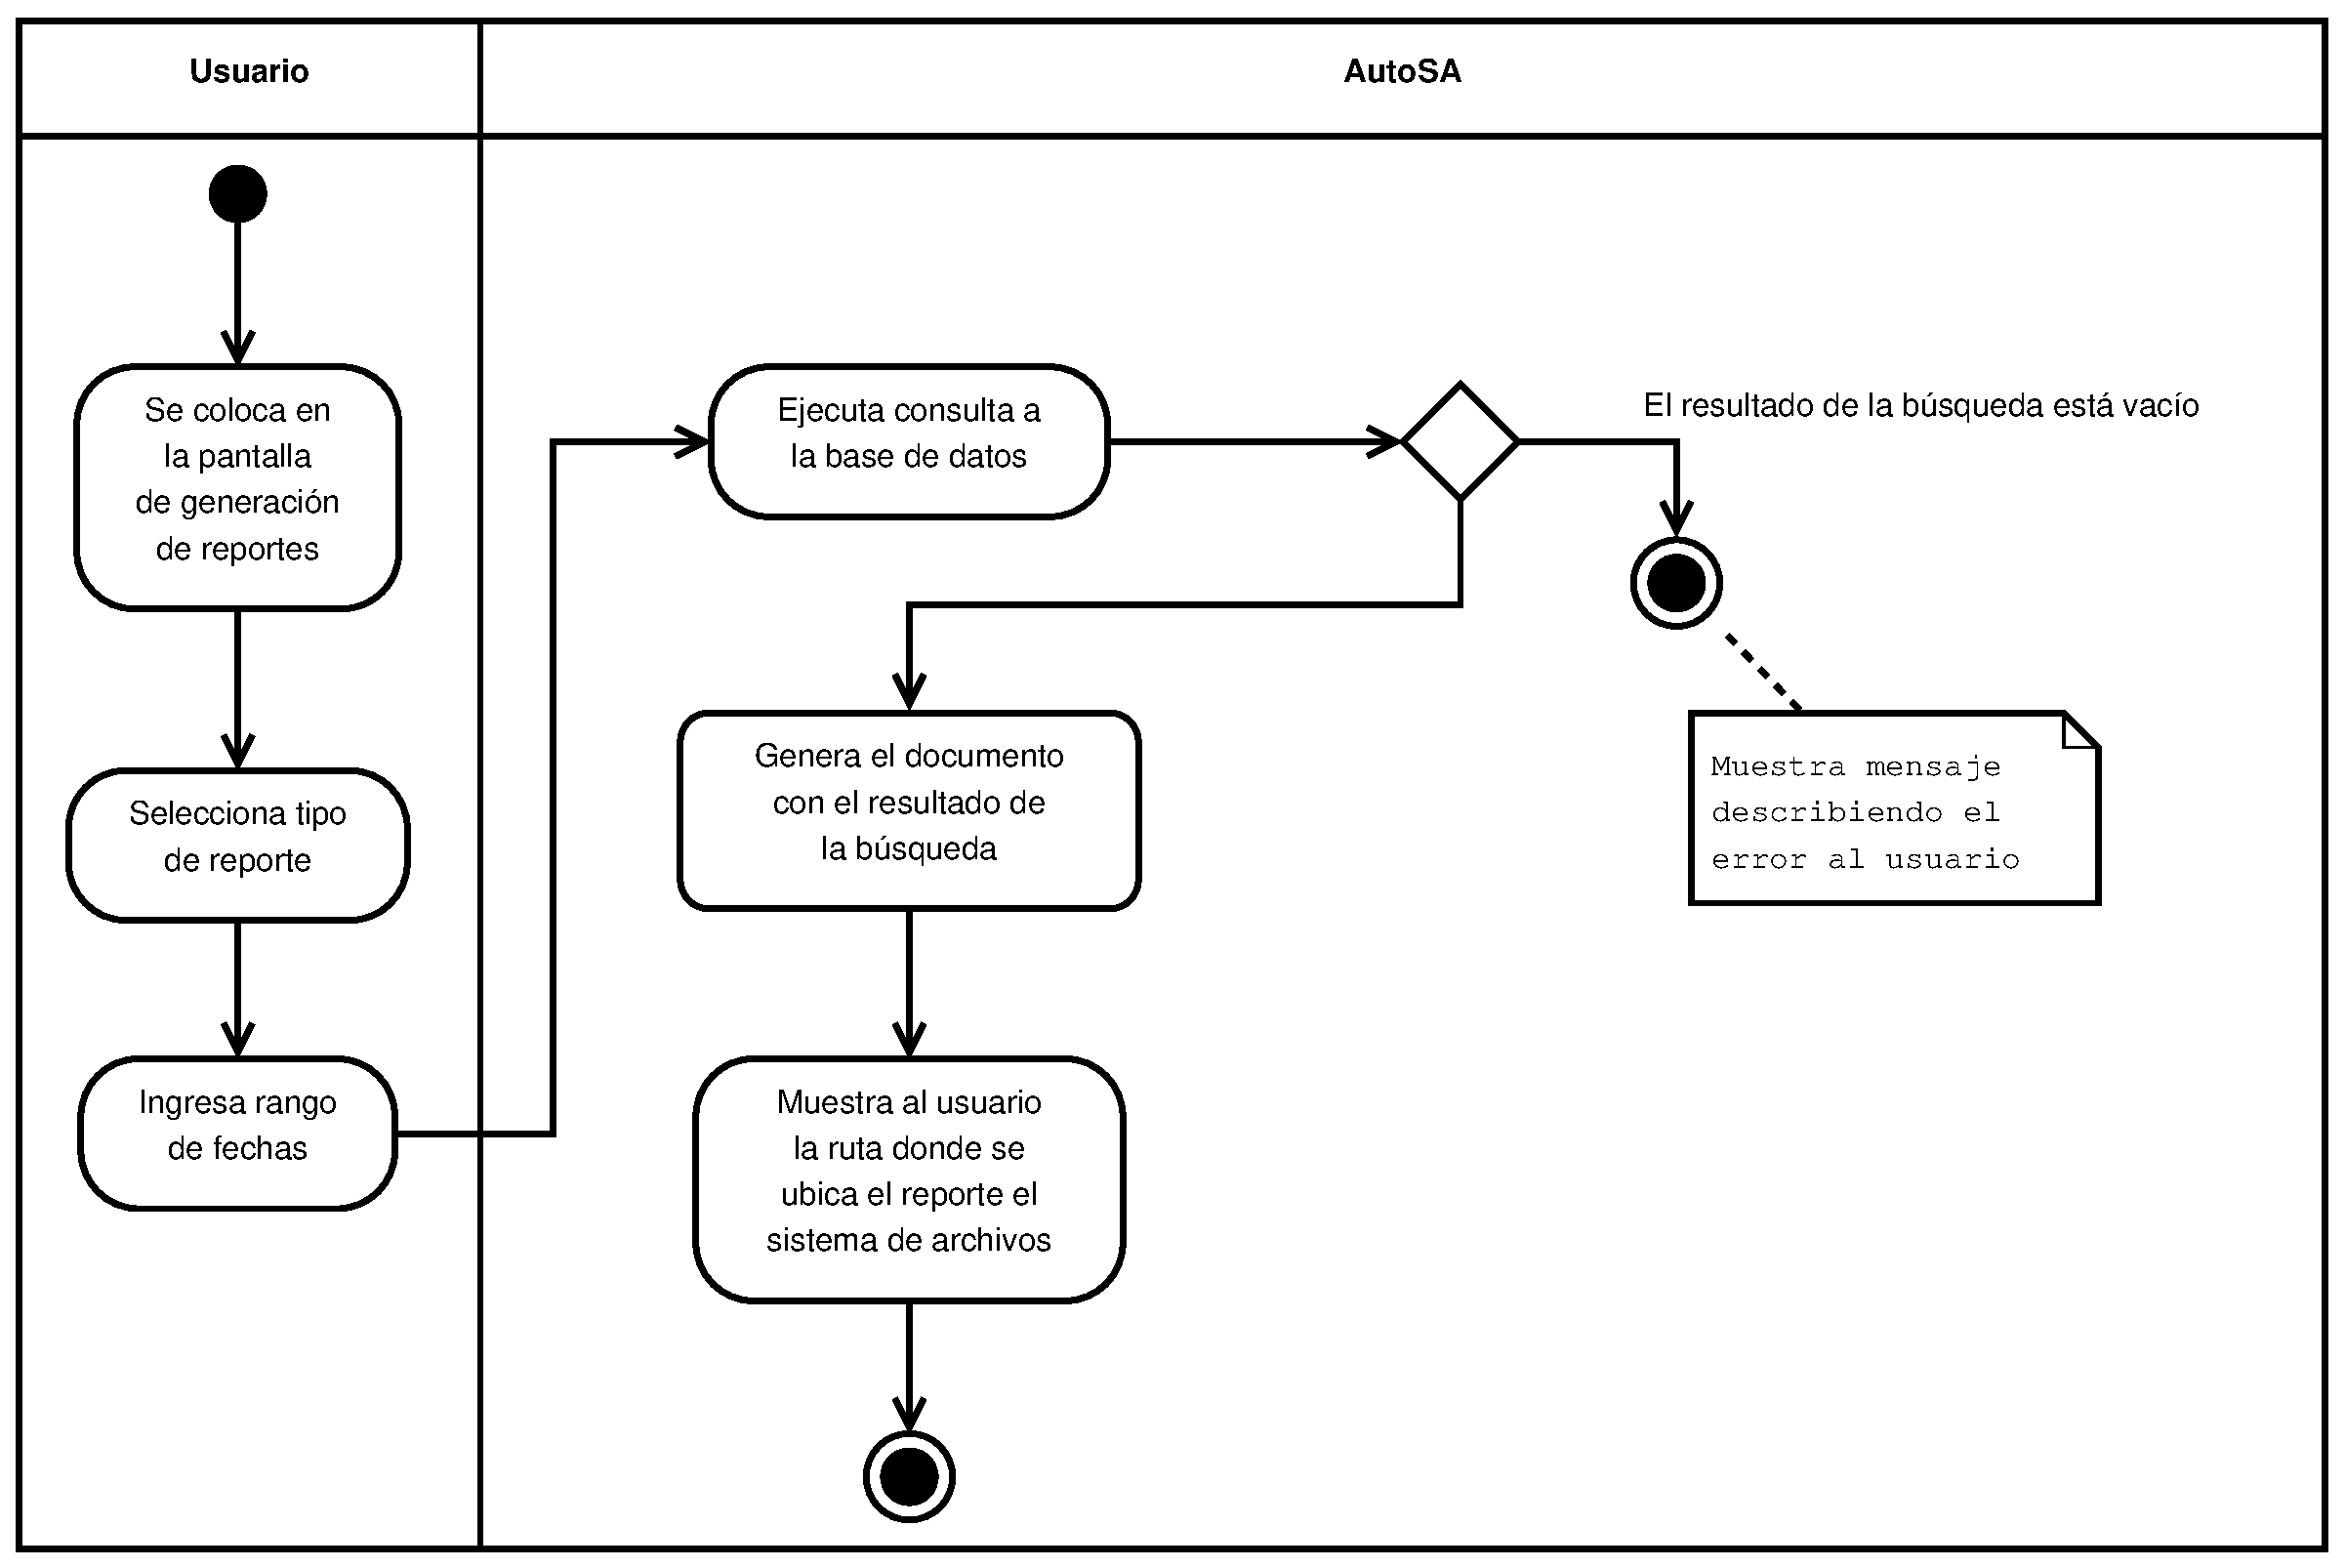
\includegraphics[width=\textwidth]{dia-activity-reporter}
  \caption{Diagrama de actividad del flujo para generación de reportes.}
  \label{fig:dia-activity-reporter}
\end{figure}
%espaciado
\pagebreak
%espaciado
\paragraph{Precondiciones:}
\begin{enumerate}
  \item El usuario ha iniciado sesión correctamente en la interfaz web (caso de uso \textbf{CU-ENTRAR-WEB}).
\end{enumerate}
\paragraph{Secuencia normal:}
\begin{enumerate}
  \item El usuario navega a la pantalla de generación de reportes.
  \item En la pantalla de generación de reportes el usuario realiza las siguientes acciones:
    \begin{enumerate}
    \item Llenar el formulario de la pantalla con los siguientes campos:
    \begin{enumerate}
      \item Tipo de reporte.
      \item Fecha y hora inicial.
      \item Fecha y hora final.
    \end{enumerate}
    \item Enviar el formulario.
  \end{enumerate}
  \item El sistema ejecuta los siguientes pasos:
  \begin{enumerate}
    \item Realiza la consulta a la base de datos definida para el reporte requerido en el paso 2.a.
    \item El resultado del paso anterior es escrito en un archivo extendido de \textit{Excel}\textsuperscript{\textcopyright} y depositado en el sistema de archivos.
    \item Muestra al usuario la ruta en el sistema de archivos donde fue depositado el reporte.
  \end{enumerate}
\end{enumerate}
\paragraph{Postcondiciones:}
\begin{enumerate}
  \item El reporte se encuentra en el sistema de archivos dentro un archivo con formato extendido de \textit{Excel}\textsuperscript{\textcopyright}.
\end{enumerate}
\paragraph{Excepciones:}
\begin{enumerate}
  \item Si el reporte no cuenta con registros el archivo no se genera y se muestra un mensaje al usuario indicando la situación.
\end{enumerate}


\subsection{Actualizar catálogo}\label{cu-actualizar-catalogo}
\paragraph{Identificador:}
CU-ACTUALIZAR-CATALOGO
\paragraph{Actores:}
Usuario
\paragraph{Descripción:}
Define la actualización masiva de los catálogos en la base de datos mediante un archivo ingresado por un usuario de la interfaz web. La Figura \ref{fig:dia-activity-cat-update} muestra el diagrama de actividad para este caso de uso, donde se puede apreciar que se inicia cuando el usuario solicita la pantalla de administración de catálogos (parte superior del apartado Usuario del diagrama de actividad).
\begin{figure}[h]
  \centering
  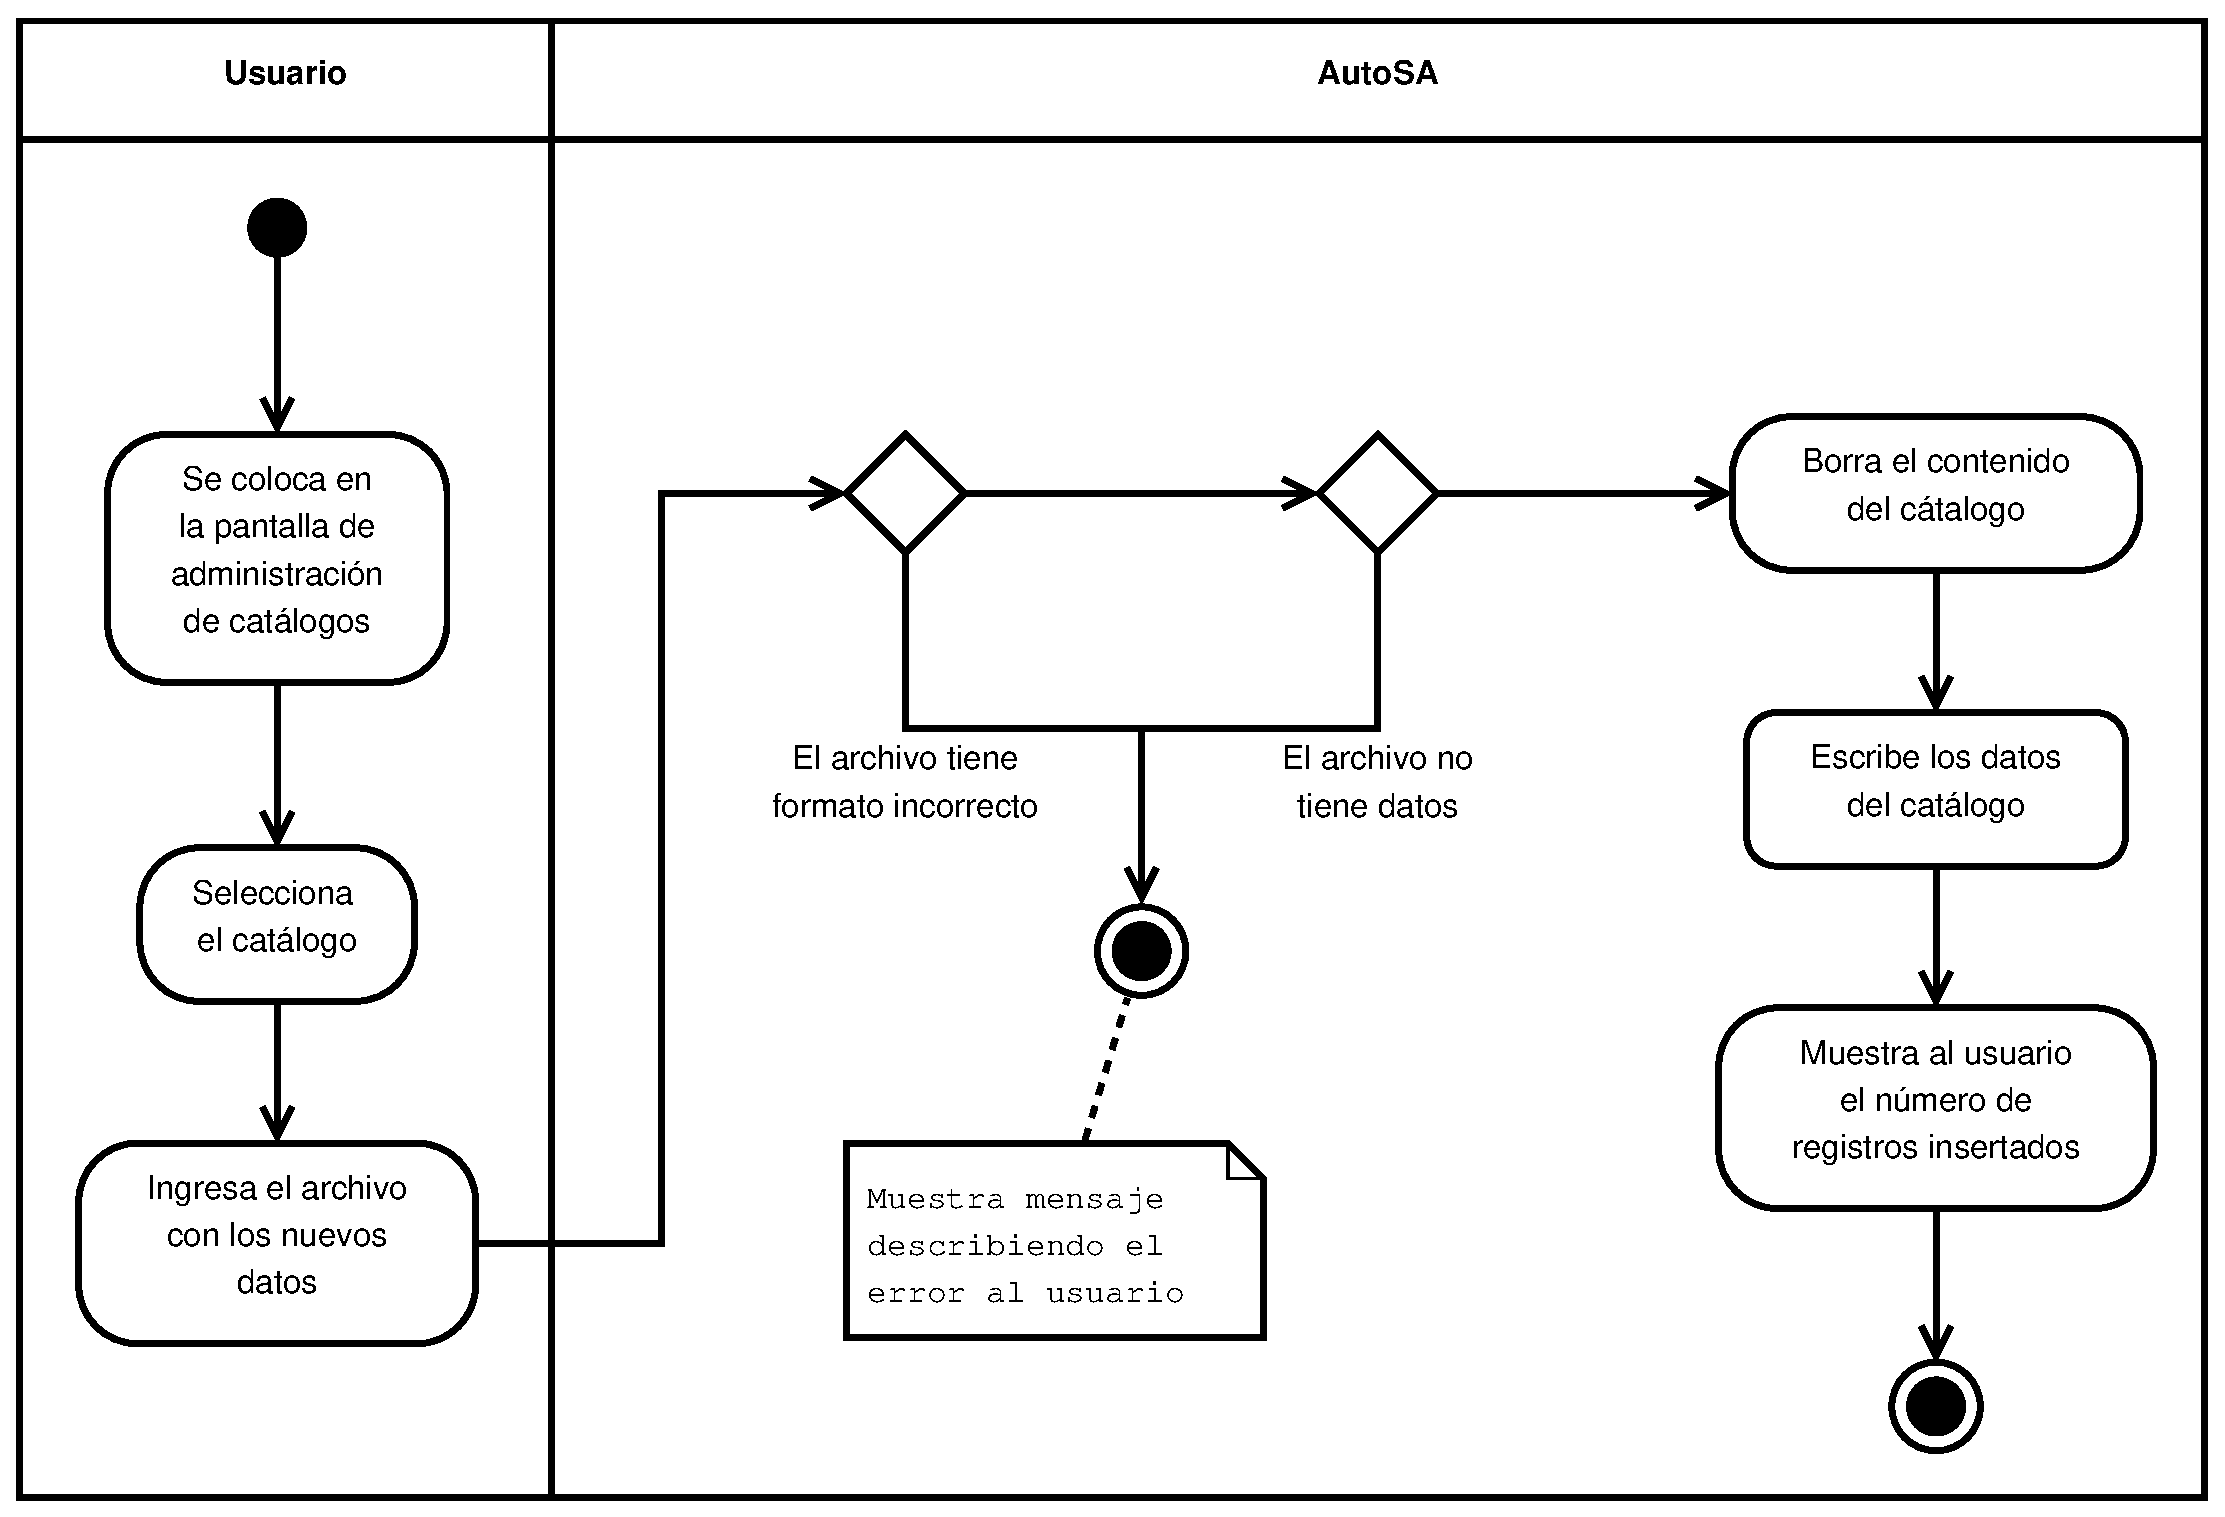
\includegraphics[width=\textwidth]{dia-activity-cat-update}
  \caption{Diagrama de actividad del flujo para la actualización de catálogos.}
  \label{fig:dia-activity-cat-update}
\end{figure}
\paragraph{Precondiciones:}
\begin{enumerate}
  \item El usuario ha iniciado sesión correctamente en la interfaz web (caso de uso \textbf{CU-ENTRAR-WEB}).
  \item El archivo ingresado tiene formato extendido de \textit{Excel}\textsuperscript{\textcopyright}.
  \item Los catálogos que pueden ser modificados por este caso de uso son aquellos que contienen códigos de medicamentos y lugares de entrega.
\end{enumerate}
\paragraph{Secuencia normal:}
\begin{enumerate}
  \item El usuario navega a la pantalla de administración de catálogos.
  \item El usuario realiza las siguientes acciones en la pantalla de administración de catálogos:
  \begin{enumerate}
    \item Seleccionar el nombre del catálogo.
    \item Seleccionar el archivo en formato de \textit{Excel}\textsuperscript{\textcopyright} que contiene la información para el catálogo.
    \item Enviar el formulario.
  \end{enumerate}
  \item El sistema sigue los siguientes pasos:
  \begin{enumerate}
    \item Valida el formato del archivo recibido.
    \item Valida que el archivo recibido contenga al menos un renglón sin contar el encabezado.
    \item Borra el contenido del catálogo en la base datos y copia la información del archivo recibido.
    \item Muestra al usuario el número de registros guardados en el catálogo después de la actualización.
  \end{enumerate}
\end{enumerate}
\paragraph{Postcondiciones:}
\begin{enumerate}
  \item El catálogo ha sido actualizado al contenido del archivo proporcionado por el usuario.
\end{enumerate}
\paragraph{Excepciones:}
\begin{enumerate}
  \item Si el archivo no cuenta con el formato solicitado, entonces se muestra un mensaje de error al usuario y se cancela la ejecución sin modificar el catálogo en la base de datos.
  \item Si el archivo no contiene ningún registro para el catálogo, entonces se muestra un mensaje de error al usuario y se cancela la ejecución sin modificar el catálogo en la base de datos.
\end{enumerate}


\subsection{Buscar órdenes}\label{cu-buscar}
\paragraph{Identificador:}
CU-BUSCAR
\paragraph{Actores:}
Usuario
\paragraph{Descripción:}
Define el flujo para la búsqueda de órdenes de reposición. La Figura \ref{fig:dia-activity-search} muestra el diagrama de actividad para este caso de uso, en ella se puede apreciar que el flujo inicia cuando el usuario solicita la pantalla de búsqueda de órdenes (parte superior izquierda) y termina cuando el sistema muestra el resultado de la búsqueda (parte inferior derecha, si la búsqueda tiene al menos una orden).
\begin{figure}[h]
  \centering
  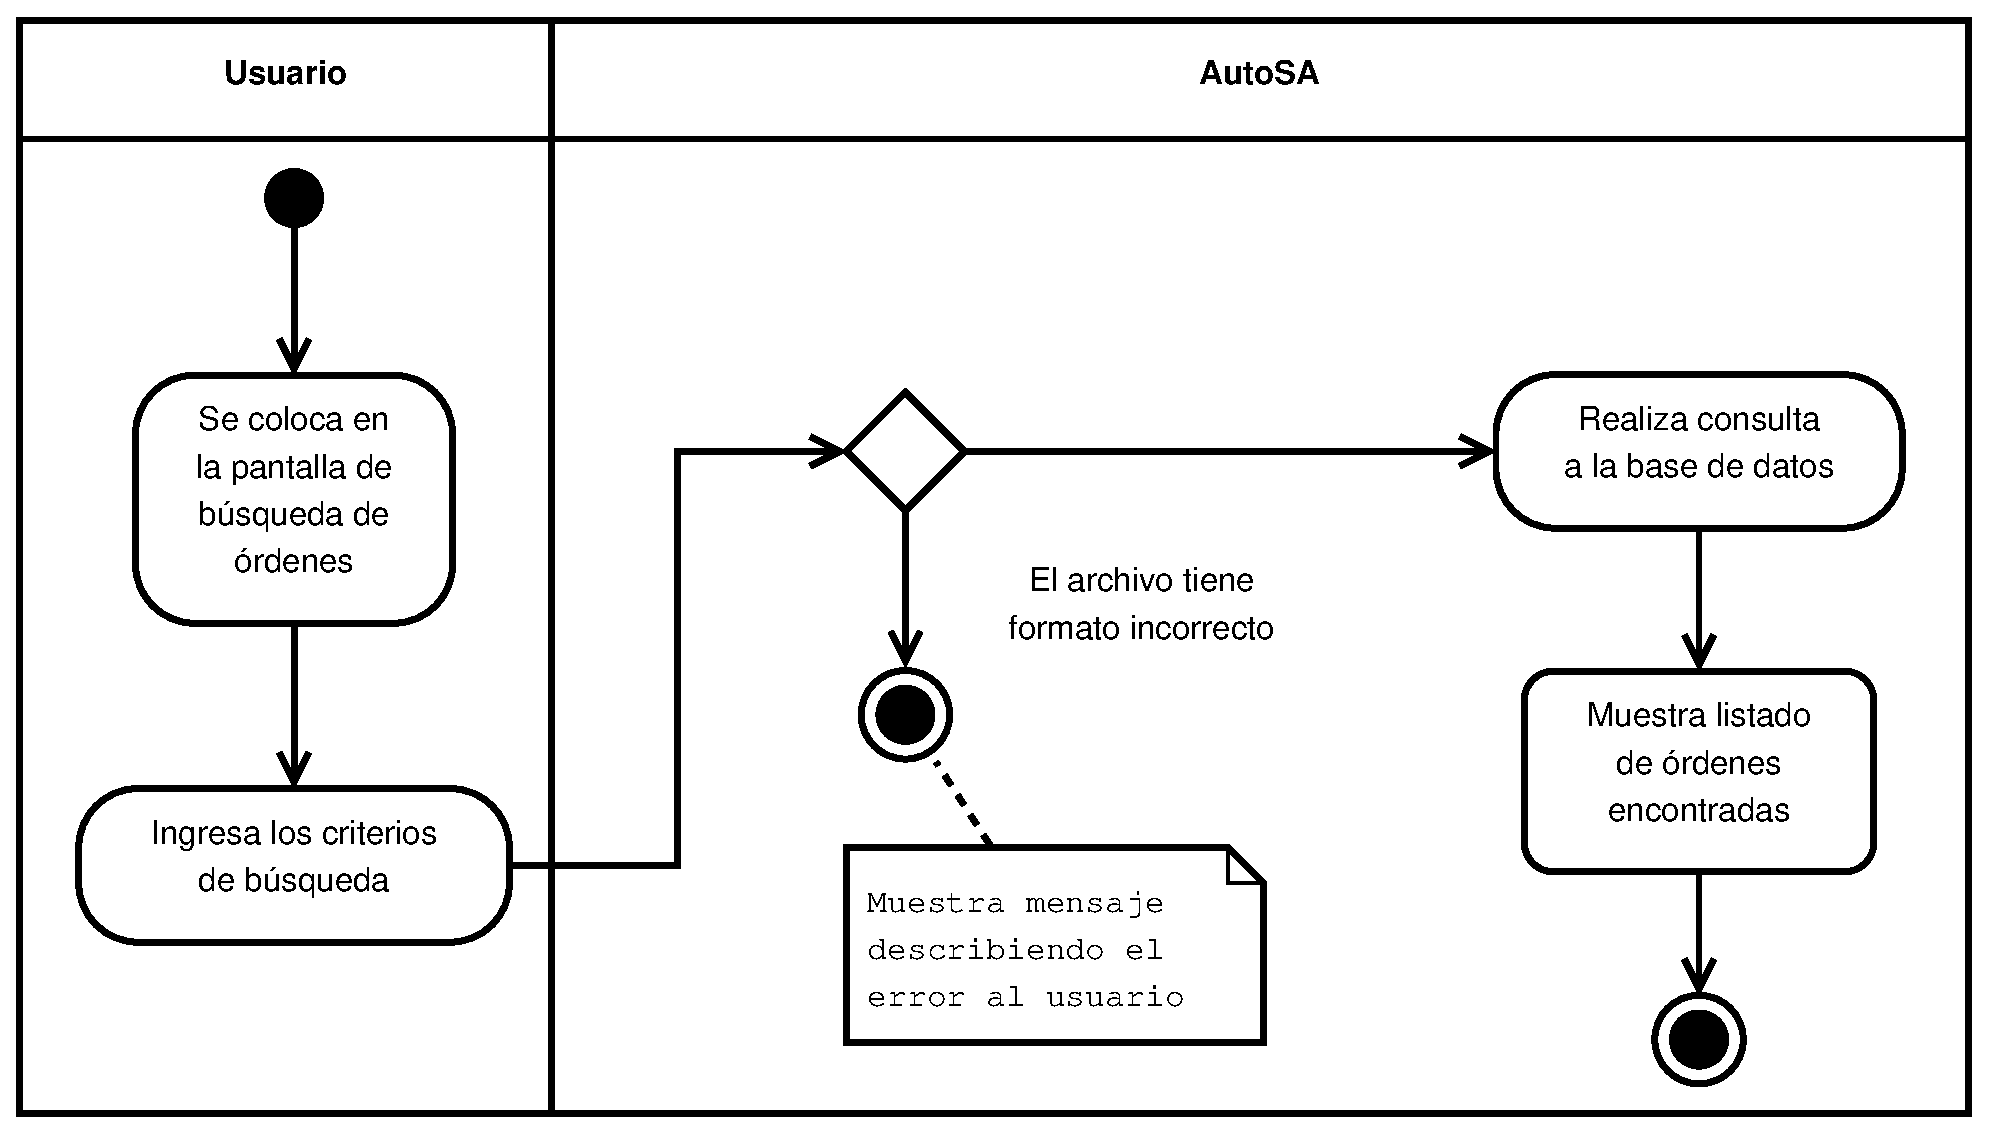
\includegraphics[width=\textwidth]{dia-activity-search}
  \caption{Diagrama de actividad del flujo para la búsqueda de órdenes de reposición.}
  \label{fig:dia-activity-search}
\end{figure}
\paragraph{Precondiciones:}
\begin{enumerate}
  \item El usuario ha iniciado sesión correctamente en la interfaz web (caso de uso \textbf{CU-ENTRAR-WEB}).
\end{enumerate}
\paragraph{Secuencia normal:}
\begin{enumerate}
  \item El usuario navega a la pantalla de búsqueda de órdenes de reposición.
  \item El usuario ingresa los criterios para la búsqueda presentados en el filtro:
  \begin{enumerate}
    \item Número de orden.
    \item Estatus de atención.
    \item Rango de fechas en que fueron atendidas las órdenes de reposición.
  \end{enumerate}
  \item El sistema muestra el resultado de la búsqueda. Para cada orden de reposición listada se muestra un enlace que lleva a la visualización de la orden (caso de uso \textbf{CU-VISUALIZAR}).
\end{enumerate}
\paragraph{Postcondiciones:}
\begin{enumerate}
  \item Se muestra un listado con las órdenes de reposición que cumplen con el filtro definido por el usuario durante el caso de uso.
\end{enumerate}
\paragraph{Excepciones:}
\begin{enumerate}
  \item En caso de no contar con una conexión con la base de datos, se muestra un mensaje de error informando al usuario.
\end{enumerate}


\subsection{Visualizar orden}\label{cu-visualizar}
\paragraph{Identificador:}
CU-VISUALIZAR
\paragraph{Actores:}
Usuario
\paragraph{Descripción:}
La forma en que el usuario de la interfaz web es capaz de visualizar los datos de una orden de reposición. En la Figura \ref{fig:dia-activity-view} se muestra el diagrama de actividad que sigue este caso de uso. Para llegar a esta sección es necesario que el usuario haya ejecutado la búsqueda de órdenes de reposición (caso de uso \textbf{CU-BUSCAR}) y seleccionado la orden para visualizar (correspondiente a las dos actividades del Usuario en el diagrama). La dependencia de este caso de uso se muestra en la Figura \ref{fig:dia-casos-uso}.
\begin{figure}[h]
  \centering
  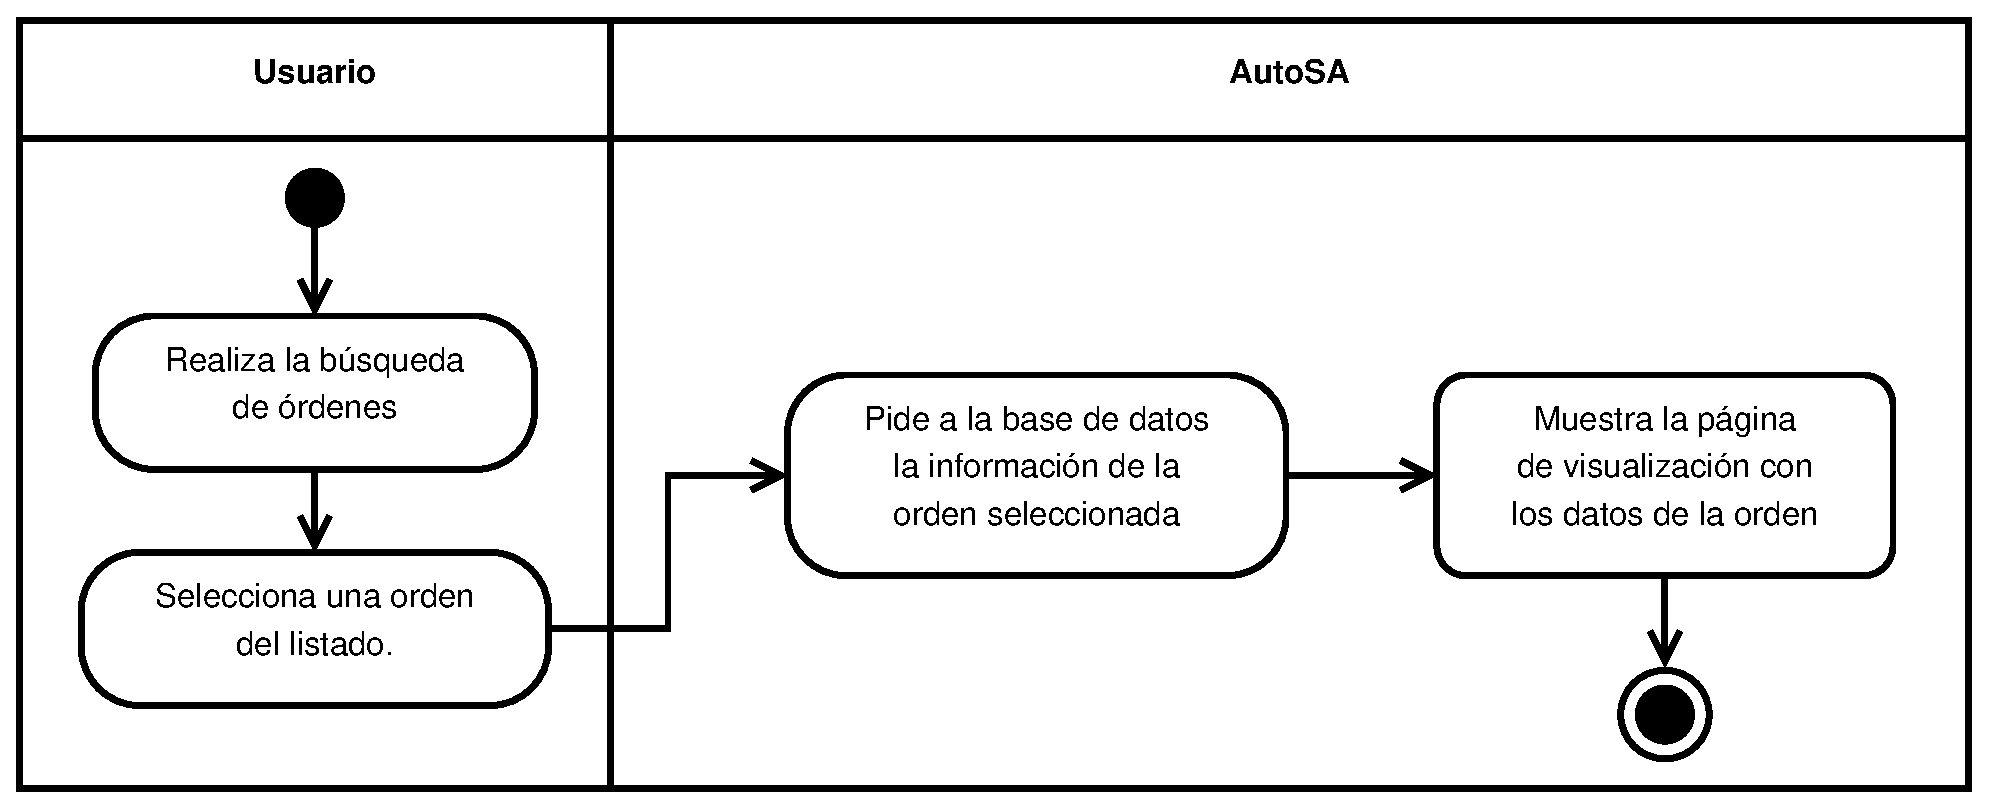
\includegraphics[width=\textwidth]{dia-activity-view}
  \caption{Diagrama de actividad del flujo para la visualización de los datos de una orden de reposición.}
  \label{fig:dia-activity-view}
\end{figure}
\paragraph{Precondiciones:}
\begin{enumerate}
  \item El usuario ha iniciado sesión correctamente en la interfaz web (caso de uso \textbf{CU-ENTRAR-WEB}).
  \item El usuario localiza la orden de reposición que desea visualizar (caso de uso \textbf{CU-BUSCAR})
\end{enumerate}
\paragraph{Secuencia normal:}
\begin{enumerate}
  \item El usuario navega a la pantalla de visualización de la orden de reposición seleccionada (caso de uso \textbf{CU-BUSCAR}).
  \item Se muestra la pantalla con los datos de la orden:
  \begin{enumerate}
    \item Se muestran todos los datos capturados del \textit{Sistema de Abastecimiento} durante el procedimiento de atención.
    \item También se muestran los estados de atención, es decir, el estado en el \textit{Sistema de Abastecimiento}  y el estado de atención en el sistema AutoSA.
  \end{enumerate}
  \item Se muestran enlaces para que el usuario pueda editar los datos de la orden (caso de uso \textbf{CU-EDITAR}) y también para generar el acuse de envío (caso de uso \textbf{CU-GENERAR-ACUSE}).
  \item En caso de seleccionar la generación del acuse de envío se ejecuta el caso de uso \textbf{CU-GENERAR-ACUSE}.
\end{enumerate}
\paragraph{Postcondiciones:}
\begin{enumerate}
  \item Se muestra una pantalla al usuario con los datos de la orden de reposición solicitada, además las opciones para editar y generar el acuse de envío.
\end{enumerate}
\paragraph{Excepciones:}
\begin{enumerate}
  \item En caso de no contar con una conexión a la base de datos se muestra un mensaje de error informando al usuario.
\end{enumerate}


\subsection{Editar orden}\label{cu-editar}
\paragraph{Identificador:}
CU-EDITAR
\paragraph{Actores:}
Usuario
\paragraph{Descripción:}
La forma en que el usuario de la interfaz web puede modificar los datos de una orden de reposición desplegada en pantalla (caso de uso \textbf{CU-BUSCAR}). En la Figura \ref{fig:dia-activity-edit} se muestra el diagrama de actividad que sigue este caso de uso. Para llegar a esta vista es necesario que el usuario haya ejecutado la visualización de la orden de reposición que desea modificar (primeras dos actividades del Usuario en el diagrama). La dependencia de este caso de uso se observa en la Figura \ref{fig:dia-casos-uso}.
\begin{figure}[h]
  \centering
  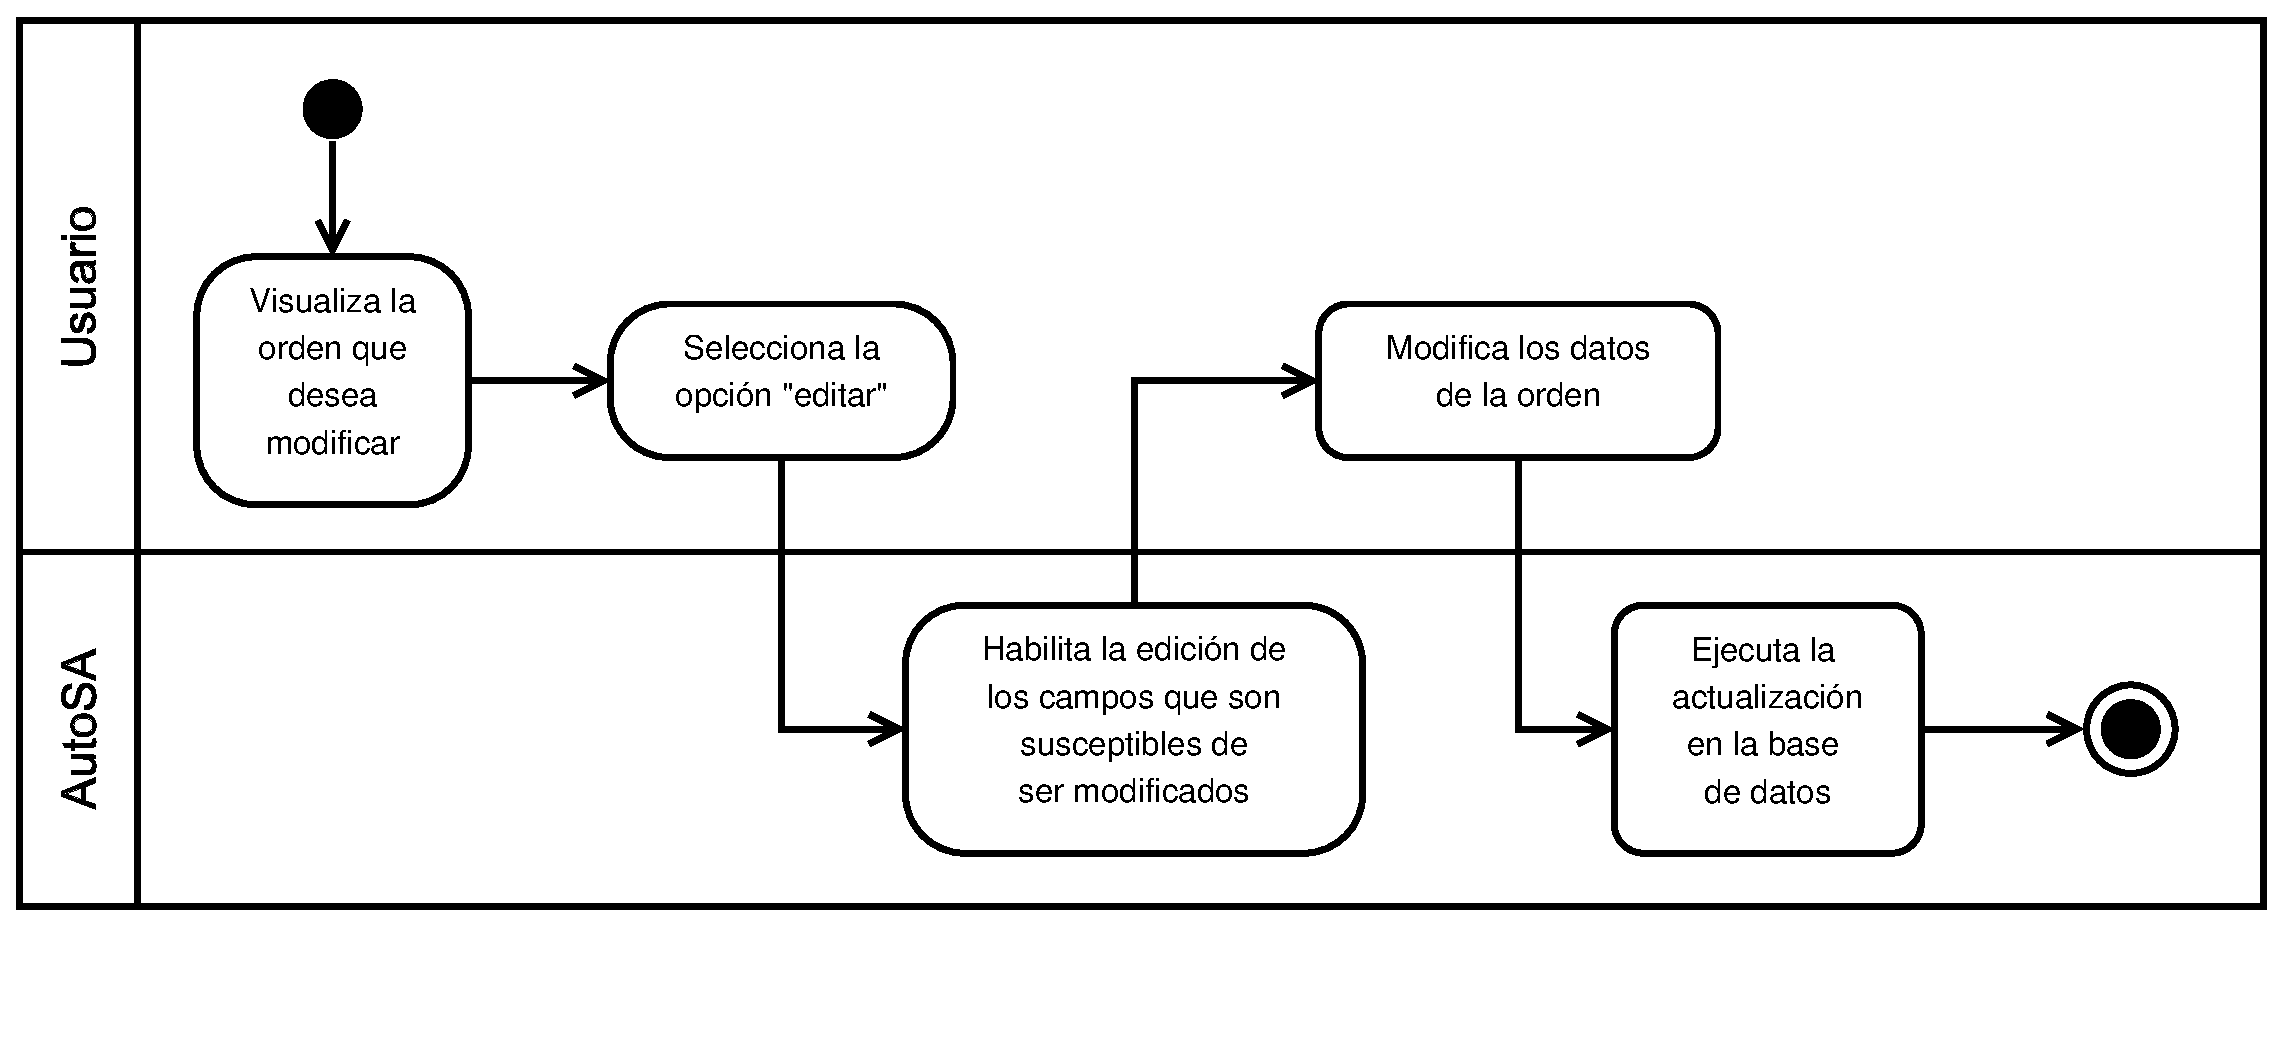
\includegraphics[width=\textwidth]{dia-activity-edit}
  \caption{Diagrama de actividad del flujo para la modificar de los datos de una orden de reposición.}
  \label{fig:dia-activity-edit}
\end{figure}
%espaciado
\pagebreak
%espaciado
\paragraph{Precondiciones:}
\begin{enumerate}
  \item El usuario ha iniciado sesión correctamente en la interfaz web (caso de uso \textbf{CU-ENTRAR-WEB}).
  \item El usuario visualiza la orden de reposición que desea editar (caso de uso \textbf{CU-VISUALIZAR}).
  \item Los campos utilizados para identificar unívocamente la orden de reposición no podrán ser modificados. 
\end{enumerate}
\paragraph{Secuencia normal:}
\begin{enumerate}
  \item El usuario navega a la pantalla de edición con la orden de reposición visualizada (caso de uso \textbf{CU-VISUALIZAR}).
  \item Cambia cualquiera de los campos modificables.
  \item Selecciona el botón Guardar.
\end{enumerate}

% espaciado
\pagebreak
% espaciado

\paragraph{Postcondiciones:}
\begin{enumerate}
  \item Los datos modificados por el usuario en la interfaz web se encuentran almacenados en la base de datos.
\end{enumerate}
\paragraph{Excepciones:}
\begin{enumerate}
  \item En caso de no contar con una conexión a la base de datos se muestra un mensaje de error informando al usuario.
\end{enumerate}

\section{Resumen}
Se ha definido el alcance del proyecto que comprende la automatización de los procesos realizados por los operadores del \textit{Sistema de Abastecimiento} hasta la generación del formato de salida, así como el alcance de la interfaz web comprende las tareas de modificación de órdenes de reposición atendidas, generación de reportes y actualización de catálogos.\\
A lo largo de este capítulo se han definido los casos de uso que reflejan el comportamiento esperado del sistema para la automatización de procesos y la interfaz web.
